\documentclass[12pt,a4paper]{article}
\usepackage[utf8]{inputenc}
\usepackage[T1]{fontenc}
\usepackage{amsmath}
\usepackage{amsfonts}
\usepackage{amssymb}
\usepackage{graphicx}
\usepackage{natbib}
\usepackage{hyperref}
\usepackage{lineno}
\usepackage{xcolor}
\usepackage{listings}
\usepackage{float}
\usepackage{pdflscape}
\usepackage{multirow}
\usepackage{longtable}
\usepackage{orcidlink}

% Configure listings package for code blocks
\lstset{
    breaklines=true,
    breakatwhitespace=false,
    columns=fullflexible,
    keepspaces=true,
    basicstyle=\ttfamily\small,
    frame=single,
    literate={°}{{$^\circ$}}1
}

\title{Data-Driven Discovery of Mechanistic Ecosystem Models with LLMs}

\author{Scott Spillias\orcidlink{0000-0002-1310-5202}\textsuperscript{1,2}\thanks{Corresponding author: scott.spillias@csiro.au} \and
Jacob Rogers\orcidlink{0000-0002-4724-2555}\textsuperscript{3} \and
Fabio Boschetti\orcidlink{0000-0001-8999-6913}\textsuperscript{2,4} \and
Beth Fulton\orcidlink{0000-0002-5904-7917}\textsuperscript{1,2} \and
Magda Guglielmo\orcidlink{0000-0002-2800-0657}\textsuperscript{5} \and
SukYee Yong\orcidlink{0000-0002-5204-2902}\textsuperscript{5} \and
Rowan Trebilco\orcidlink{0000-0001-9712-8016}\textsuperscript{1,2}
}

\date{\today}

\newcommand{\keywords}{%
Artificial Intelligence,
Ecological modelling,
Evolutionary Algorithms,
Large Language Models,
Marine Ecosystems,
Crown-of-Thorns Starfish,
Great Barrier Reef,
time-series forecasting%
}

% Author affiliations
\newcommand{\affiliations}{
\noindent\textsuperscript{1}CSIRO Environment, Hobart, Australia\\
\textsuperscript{2}Centre for Marine Socio-Ecology, University of Tasmania, Hobart, Australia\\
\textsuperscript{3}CSIRO Environment, St. Lucia, Australia\\
\textsuperscript{4}CSIRO Environment, IOMRC Crawley, Australia\\
\textsuperscript{5}CSIRO IM\&T, Eveleigh, Australia\\
}

\begin{document}
% \linenumbers
\maketitle
\affiliations
\vspace{1em}

\noindent\textbf{Keywords:} \keywords
\vspace{2em}
\newpage
\begin{abstract}
Ecosystem models are essential for ecosystem management, but their development traditionally requires significant time and expertise, creating bottlenecks in addressing urgent environmental challenges. We integrate large language models (LLMs) with evolutionary optimization to automate the discovery of interpretable ecological models from time-series data. Our framework `LEMMA' (LLM-Enabled Mechanistic Modelling for ecosystem Assessment) addresses the inverse problem of inferring ecologically meaningful mechanistic models that explain observed data while maintaining biological plausibility. We critically review LEMMA's ability to recover known ecological relationships through two complementary marine case studies: (1) a nutrient-phytoplankton-zooplankton model, and (2) a Crown-of-Thorns starfish (COTS) model. In the first case, our best models displayed almost perfect recovery of known ecological dynamics while maintaining strong predictive performance across multivariate time-series. In the second case, best LEMMA generated models approached human expert models in terms of their ability to successfully capture COTS outbreak dynamics and demonstrated strong out-of-sample predictive power. LEMMA produces interpretable models with meaningful parameters that capture real biological processes, facilitating scientific insight and potentially accelerating management applications. By dramatically accelerating model development while offering ecological interpretability, LEMMA offers a powerful new tool for addressing urgent ecological challenges in rapidly changing environments.
\end{abstract}

\section{Introduction}
Ecosystem models provide invaluable information for managing complex interactions between nature and people \citep{McCarthy2004, Holden2016}, but their development traditionally requires significant time and expertise, creating a bottleneck in addressing urgent environmental challenges \citep{Dichmont2017,Holden2024b}, particularly as climate change demands rapid, adaptable approaches for ecosystem management \citep{weiskopf2020climate,malhi2020climate}.

Artificial Intelligence (AI) offers great promise as a part of the solution to these modelling challenges, with potential to accelerate model development and enhance adaptability \citep{Spillias2024}. While initial efforts to apply AI in ecological modelling focused on machine learning approaches that rely on black-box methods \citep{morales2024developing}, emerging techniques in equation discovery and automated scientific discovery show particular promise \citep{Huntingford_Nicoll_Klein_Ahmad_2024,floryan2022data}. These methods can derive interpretable mathematical relationships directly from data, offering advantages over statistical emulators when modelling novel environmental conditions \citep{Schaeffer_2017,chen2024constructing,karniadakis2021physics}. Similarly, attempts to leverage large language models (LLMs) for direct time-series prediction \citep{zhang2024large,su2024large,hassani2024predictions,gandhi2024generative,bylund2024chatgpt,cao2023tempo,li2024lite,garza2023timegpt}, though successful in other fields, are unsuited for producing reliable ecological insights or testing management interventions. For instance, work on multimodal LLMs for environmental prediction \citep{li2024lite} achieves impressive accuracy in forecasting physical variables like streamflow and water temperature, but does not address the mechanistic relationships needed for ecosystem management and applications.

Rather than using AI to replace traditional modelling approaches, recent advances in AI coding capabilities suggest a more promising direction \citep{Xu2021}. Language models like o3-mini and Claude can assist in constructing mechanistic models \citep{Spillias2024}, maintaining interpretability while accelerating the development process \citep{TheRoyalSociety2024}. Recent demonstrations of LLMs automating scientific processes, from autonomous chemical experimentation \citep{burger2023autonomous} to biomedical research \citep{wang2024bioresearcher}, evidence synthesis \citep{spillias2024evaluating} and even fully automated scientific discovery \citep{kramer2023automated}, highlight their potential for systematic scientific work. The key challenge lies in developing frameworks that can systematically harness these capabilities while ensuring scientific rigor and maintaining human oversight in the discovery process \citep{kramer2023automated,Spillias2024}. To the best of our knowledge, such an approach has not been attempted yet in ecological modelling.

To address this challenge, we present ``AI for Models of Ecosystems'' (AIME), a novel framework that requires minimal inputs, only time-series data and research questions, and aims to produce ecologically sound mathematical models that explain the time-series data (Figure \ref{fig:modelling_intro}). AIME addresses the inverse problem of inferring ecologically meaningful mechanistic models and parameters that causally explain observed data. The inferred models can then be used to test management interventions and scenarios. When solving inverse problems through numerical optimization, practitioners usually predetermine the model and its allowable parameter ranges, which defines both the parameter space and its mapping to the observation space. Less commonly, the model itself is inferred directly from observations, as in Scientific Machine Learning (SciML), System Identification, and Automated Algorithm Discovery. Successful model reconstruction in such scenarios requires extensive data to ensure statistical relations are represented in the observations. In addition, a common challenge across all inverse problem approaches is the need to impose constraints that prevent numerically accurate yet empirically unrealistic solutions. AIME differs from traditional and SciML approaches by leveraging information available to current LLMs to impose ecologically meaningful constraints on both forward models and parameter ranges. This addresses the significant limitation of sparse ecological observations. Within this framework, AIME employs Template Model Builder (TMB, a R/C++ library for efficient parameter estimation in complex nonlinear models) as its foundation, providing a rigorous statistical framework for ecological modelling. The system operates through an iterative process where an LLM generates candidate model structures as TMB-compatible equations, which are then evaluated against time-series data using normalized objective functions (where lower values indicate better model fit). These models undergo evolutionary optimization across multiple generations, where successful structures (referred to as ``individuals'') are selected and improved upon, while underperforming models are culled. This evolutionary approach systematically produces increasingly accurate representations of ecosystem dynamics and offers a way to explore relative support for multiple possible mechanistic structures.

We test AIME's ability to construct plausible ecological models through two complementary case studies that test different aspects of ecological modelling, each involving both dependent variables (state variables predicted by the model) and forcing variables (external drivers affecting the system). First, we evaluate the framework's ability to recover fundamental ecological understanding using synthetic data generated from a well-established nutrient-phytoplankton-zooplankton (NPZ) model \citep{edwards1999zooplankton}.  This controlled experiment tests AIME's equation-learning capabilities by comparing discovered equations against known mathematical relationships that represent core ecological processes. For our NPZ case study, we additionally evaluate models using ecological accuracy scores (on a scale of 0-8), which measure how well the generated models recover known ecological mechanisms from the reference model. These scores assess specific components like nutrient uptake, phytoplankton growth, and zooplankton dynamics, with higher scores indicating closer alignment with established ecological understanding. Second, we assess AIME's ability to provide management-relevant predictions using synthetic data based on Crown-of-Thorns starfish (COTS) populations on the Great Barrier Reef, derived from existing MICE models \citep{Morello_Plaganyi_Babcock_Sweatman_Hillary_Punt_2014, Rogers_Plaganyi_2022,Plaganyi_Punt_Hillary_Morello_Thebaud_Hutton_Pillans_Thorson_Fulton_Smith_et_al_2014, Condie_Anthony_Babcock_Baird_Beeden_Fletcher_Gorton_Harrison_Hobday_Plaganyi_et_al_2021}. The COTS case study, with three dependent variables (COTS abundance, fast-growing coral cover, and slow-growing coral cover) and two forcing variables (temperature and COTS immigrants), tests the framework's robustness while focusing on a specific management challenge: quantifying outbreaks in a complex predator-prey system. Through systematic comparison of different LLMs (o3-mini, o4-mini, and GPT4.1 from OpenAI, Claude Sonnet 3.7 and 3.7 from Anthropic, and Gemini from Google), we evaluate how different AI capabilities affect model performance. This comparative approach demonstrates how our evolutionary framework can both recover theoretical ecological relationships and are potentially suitable for use in support of ecosystem management.

\begin{figure}[H]
    \centering
    \includegraphics[width=0.8\textwidth]{../Figures/modelling_steps_AI_&_human}
    \caption{Stylised representation of the iterative modelling process that AIME aims to support. Whilst human experts drive the majority of the process, we show that AI-driven processes could play an important role in the Model Development stage.}
    \label{fig:modelling_intro}
    \end{figure}
\section{Methods}
At its core, LEMMA integrates Large Language Models (LLMs) for generating and modifying model structures, Template Model Builder (TMB) for statistical parameter estimation, and evolutionary algorithms for systematic model improvement. All of the code and data underpinning this study are available at the Github repository: \url{https://anonymous.4open.science/r/EMs-with-LLMs-10E8}.

\subsection{LEMMA Framework}

\subsubsection{Model Generation and Improvement}
LEMMA uses LLMs to write and modify computer code through Aider \citep{gauthier2024aider}, which is a coding assistant that can create, modify, and interpret local files. Aider can be used in the command-line or called within python scripts, as we have done here, and can receive text and/or images as input, depending on whether the underlying LLM is 'multi-modal' (i.e., can interpret text and images). Each model instance, referred to as an individual in our evolutionary framework, consists of three components: (1) a TMB-compatible dynamic model written in C++ that implements a system of equations, (2) a parameters file containing initial values and bounds, and (3) a documentation file explaining the ecological meaning of the model equations (see Section \ref{subsec:initial_model_prompt} for the complete prompt).

The LLM generates initial parameter estimates for pre-testing model structure before optimization begins. For each parameter, it assigns a priority number that determines optimization order, following established practices in ecosystem modelling \citep{Plaganyi_Punt_Hillary_Morello_Thebaud_Hutton_Pillans_Thorson_Fulton_Smith_et_al_2014}.

During non-initial steps, if multi-modal (i.e. can receive images as input) the LLM analyzes performance plots comparing predictions to historical data, otherwise the LLM receives a structured file showing the model fit residuals. After interpreting the model fit, LEMMA makes targeted, ecologically meaningful changes to model equations, implementing one modification at a time to maintain transparency and traceability of successful modelling strategies (see Section~\ref{subsec:model_improvement_prompt}).

\begin{landscape}
    \begin{figure}[p]
    \centering
    \includegraphics[width=0.85\linewidth]{../Figures/conceptual_diagram}
    \begingroup
    \small
    \caption{Conceptual diagram of the automated ecological modelling framework, LEMMA. The workflow consists of five main components: (1) User Inputs, where research questions and ecological time-series data are provided; (2) Parameterisation, utilizing RAG-enhanced literature search to estimate parameter values; (3) Model Generation/Improvement, where the Coding LLM creates new individuals with model scripts and parameters; (4) Model Execution, where the LLM's model code is implemented and TMB is used to optimise parameter values; and (5) Evolution, which evaluates model performance through individual assessment, error handling, and ranking-based selection.}
    \label{fig:conceptual}
    \endgroup
    \end{figure}
    \end{landscape}

\subsubsection{User Inputs}

The LEMMA framework requires only minimal user input to initiate the modelling process. At the outset, the user provides a short natural language description of the ecological system and research question, which guides the large language model (LLM) in generating ecologically relevant model structures. Two time-series data files are also supplied: a response file containing the dependent variables (state variables) to be predicted by the model, and a forcing file containing external drivers that influence system dynamics. Column headers in these files define the variables that are directly observed and available for model fitting. Importantly, the framework is not restricted to these variables; the LLM may introduce additional latent variables or intermediate processes when such constructs are ecologically justified and improve model performance. This flexibility allows LEMMA to explore a broader range of mechanistic hypotheses than would be possible if limited to observed variables alone.

In addition to these core inputs, users may optionally specify configuration parameters that control the evolutionary process and LLM behaviour, including the sampling temperature, the number of individuals per generation, the number of generations, the convergence threshold, and the proportion of data allocated to training versus testing. Users also select the LLM for code generation, the model for literature retrieval, and the embedding model for semantic search. Finally, the user can specify a directory with curated ecological literature from which LEMMA will identify plausible parameter values and bounds. These inputs collectively define the modelling context while allowing LEMMA to operate with minimal manual intervention and substantial flexibility in model structure.

\subsubsection{Parameterisation}
Upon initialization, the LLM estimates parameter values for each parameter in its proposed model. LEMMA uses this initial estimation to quickly run the model using TMB to identify structural or syntactical errors in the LLM-generated code. If a candidate model is successful in compiling and running, LEMMA refines these estimates using evidence from the scientific literature. Building on the success of LLM-based extraction from ecological literature \citep{keck2025extracting,spillias2024evaluating}, LEMMA implements a RAG architecture to search scientific literature (see Section~\ref{subsec:rag_architecture} for detailed RAG implementation). Without this initial estimation step, LEMMA risks wasting time and computational resources searching for parameter values to populate equations that may be structurally or syntactically flawed.

The RAG process works as follows: First, LEMMA prompts an LLM to create detailed semantic descriptions of each parameter, expanding beyond the basic descriptions provided by the coding LLM. For example, if the coding LLM defines a parameter as ``growth rate of phytoplankton,'' the RAG system might expand this to ``maximum specific growth rate of marine phytoplankton in nutrient-rich conditions, measured per day.'' These enhanced descriptions aim to improve the relevance of search results when querying literature databases.

To find appropriate parameter values, the RAG system employs a structured, multi-source search strategy. It searches a curated local collection of scientific papers (see Section~\ref{subsec:curated_literature}), queries the Semantic Scholar database \citep{semantic_scholar_api}, and performs general web searches through the Serper API \citep{serper_api}. LEMMA combines results from all three sources to build a comprehensive understanding of each parameter's possible values and ecological meaning.

The RAG system then uses LLMs to extract numerical values from the search results, determining not only parameter values but also their valid ranges. The prompt instructs the LLM to identify minimum, maximum, and typical values for each parameter, along with their units and citation information (see Section~\ref{subsec:parameter_enhancement_prompt}). All parameter information is stored in a structured database that includes bounds, units, and citations. 

\subsubsection{Model Execution, Optimisation, and Error Handling}

\paragraph{Model Execution.}
Models are executed through TMB \citep{kristensen2014tmb}, which uses automatic differentiation to efficiently compute gradients for complex, non-linear optimisation problems. The dynamically generated TMB template defines the objective function internally; LEMMA treats this as a black box and does not modify its structure. We use a Control File in \textit{R} which provides the data, starting values, and explicit box constraints for optimisation.

\paragraph{Optimisation Strategy.}
Parameter estimation proceeds in phases: parameters are grouped by LLM-assigned priority, and only those assigned to the current phase are estimated while others remain fixed. After all phases are complete, a final optimisation is performed with all parameters free. This phased approach improves stability and convergence for high-dimensional models. For this proof-of-concept, all parameters are treated as estimable in the optimisation process. The optimiser used is \texttt{nlminb}, which minimises the objective function exposed by the TMB template. Lower and upper bounds for each parameter are applied as explicit box constraints at the optimiser level. Starting values and bounds are constructed from literature-derived values when available; otherwise, LLM-estimated fallbacks are used. Before optimisation, starting values are clamped to the admissible box, and pathological intervals are normalised (swapping if lower\,$>$\,upper and expanding zero-width intervals by a small $\varepsilon$). These checks ensure numerical stability and prevent infeasible parameter configurations.

The optimisation is not iterative in epochs; instead, it uses a gradient-based solver that terminates when one of its convergence criteria is met: (a) gradient norm below tolerance; (b) parameter updates below tolerance; or (c) maximum iterations reached (default in \texttt{nlminb} is 150 iterations per phase). These stopping conditions are controlled internally by \texttt{nlminb} and are not manually tuned.

Because the TMB template is dynamically generated, LEMMA does not impose a fixed likelihood structure but assumes that the function represents a valid statistical model. The optimisation uses a maximum likelihood framework, leveraging TMB’s automatic differentiation to compute gradients. No regularisation terms are added by LEMMA; the optimisation is unconstrained beyond the explicit parameter bounds. LLM- and literature-provided values are used only to set starting points and bounds, not as penalties in the objective function.

\paragraph{Error Handling.}
Because LLMs often make trivial mistakes in their outputs, we developed an error handling system to address common issues and preserve LLM-progress, rather than discarding partial attempts. For example, on occasion, the LLM coder will attempt to create a system of equations with circular logic (``data leakage''), or will omit a key output variable with a corresponding time-series. To prevent this, we implement code validation checks to ensure that the submitted model is properly formatted and free from logical inconsistencies. For models that fail, LEMMA addresses compilation errors through automated analysis of error messages and implementation of appropriate fixes. For numerical instabilities, LEMMA employs progressive simplification of model structure while maintaining ecological relevance. Each model variant receives up to a user-specified number of fixes (five for our case-studies), with later iterations prompting for simpler model structures that can be iteratively improved. The specific prompts used for error handling are provided in Section~\ref{subsec:error_handling_prompt}.

\subsubsection{Model Evaluation}

For each response variable $j$, we calculate a normalized mean squared error:

\begin{equation}
    \text{NMSE}_j = \begin{cases}
        \frac{1}{n} \sum_{i=1}^{n} \left(\frac{y_{ij} - \hat{y}_{ij}}{\sigma_j}\right)^2 & \text{if } \sigma_j \neq 0 \\
        \frac{1}{n} \sum_{i=1}^{n} (y_{ij} - \hat{y}_{ij})^2 & \text{if } \sigma_j = 0
    \end{cases}
\end{equation}

where $y_{ij}$ represents observed values for variable $j$ at time $i$, $\hat{y}_{ij}$ represents corresponding model predictions, $\sigma_j$ is the unbiased standard deviation of the observed values for variable $j$ (calculated with $n-1$ denominator), and $n$ is the number of observations. The final objective function value is the mean across all response variables:

\begin{equation}
    \text{Objective} = \frac{1}{m} \sum_{j=1}^{m} \text{NMSE}_j
\end{equation}

where $m$ is the number of response variables. NMSE was selected as the primary objective function because it normalizes error by the standard deviation of each time-series, ensuring that all variables contribute equally to model evaluation. This avoids bias toward variables with larger magnitudes and supports balanced optimization across multivariate ecological datasets. For simplicity in this proof-of-concept, we did not weight the time-series in the objective function, however this might prove useful in future work to prioritize uncovering key dynamics.

\subsubsection{Evolutionary Algorithm Implementation}

LEMMA maintains a population of model instances, which we refer to as `individuals', where each individual represents a complete model implementation including its equations, parameters, and performance metrics. Within each generation, individuals undergo parameter optimization using Template Model Builder to find optimal parameter values for their current model structure. 

After parameter optimization, individuals are evaluated based on their prediction accuracy. Those achieving the lowest prediction errors (objective values) are selected to become parents for the next generation, while less well-performing individuals are culled and non-functioning ones (those that fail to compile or execute) are discarded. 

At the beginning of each new generation, LEMMA creates new individuals in two ways: by making targeted structural modifications to the best-performing parent individuals from the previous generation, and by creating entirely new individuals from scratch when there are not enough functioning individuals. Both of these are done via Aider's underlying tool handling routines that enable file modifications and creations and are determined by the underlying LLM's response to the standard prompts, the project topic, and the current model performance (if modifying an existing model).

\subsection{Validation Experiments}

We conducted two complementary validation case studies of LEMMA. The first validation experiment aimed to see if LEMMA could recover known model equations from synthetic time-series data, whilst the second validation experiment examined real-world applicability through modelling ecological dynamics on the Great Barrier Reef. In addition to the primary experimental design (training on the full dataset), we conducted a supplementary temporal hold-out evaluation for the COTS case study using the best-performing LLM, with three replicate populations, to assess out-of-sample predictive performance.

\subsubsection{LLM Configuration and Experimental Design}

We utilized three leading-edge LLMs to drive LEMMA's model generation and improvement processes: GPT-5, Sonnet-4.5, and Gemini-Pro-2.5. These models were selected as they represent the current state-of-the-art in language model capabilities at the time of analysis. All models were accessed via OpenRouter, and the analysis was conducted in October 2025. To maintain consistency and reduce complexity in outcomes, we employed GPT 4.1 as a dedicated support model for all parameter estimation and RAG-related queries across all three main LLMs. This approach ensured that differences in model performance could be attributed to the core model generation capabilities rather than variations in parameter retrieval or literature search processes.

To systematically evaluate LEMMA's performance across different LLMs and ecological systems, we implemented a balanced factorial experimental design. The design consisted of three replicates for each combination of the three LLMs and the two ecological case studies (NPZ and COTS). This yielded a target of 18 populations (3 LLMs $\times$ 2 case studies $\times$ 3 replicates).

Each population was initialized with four individuals and allowed to evolve for a target of ten generations, unless convergence was reached earlier (defined as achieving an objective value improvement of less than 0.01 for three consecutive generations).

\subsubsection{Retrieving Model Equations -- NPZ Case Study}

We conducted a controlled experiment using synthetic time-series data generated by a well-established nutrient-phytoplankton-zooplankton (NPZ) model from \cite{edwards1999zooplankton}, whose dynamics are well-studied \citep{boschetti2008mapping,boschetti2010detecting}. The complete system of equations is presented in Section~\ref{subsec:npz_evaluation_prompt} of the Supplementary Information. This validation tested our framework's ability to rediscover established ecological relationships from synthetic data where the underlying equations of a system are known, providing a rigorous assessment of the system's equation-learning capabilities.

In addition to monitoring the convergence of LEMMA's modelled time-series towards the provided time-series data, we evaluated the framework's ability to recover nine key ecological characteristics from the original model. These characteristics were organized by equation: three components in the nutrient equation (dN/dt: uptake, recycling, mixing), four components in the phytoplankton equation (dP/dt: growth, grazing loss, mortality, mixing), and two components in the zooplankton equation (dZ/dt: growth, mortality).

During evolution, for each `best performer' in a generation, we used GPT-5-mini to evaluate each model component using a 4-level ordinal scoring system designed to be interpretable and verifiable by ecological experts:

\begin{itemize}
    \item TRUTH\_MATCH: The mathematical structure is equivalent to the ground truth NPZ model
    \item ALTERNATE: The implementation matches a recognized alternate formulation from the ecological literature (e.g., different functional response curves from \citep{franks2002npz})
    \item SIMILAR\_NOT\_LISTED: The implementation plays the same ecological role but uses a form not represented in the ground truth or literature catalog
    \item NOT\_PRESENT\_OR\_INCORRECT: The ecological component is missing or cannot be identified
\end{itemize}

Each characteristic was assigned a weight based on its contribution to its parent equation (e.g., the three nutrient equation components each had weight 0.333, the four phytoplankton components each had weight 0.25, and the two zooplankton components each had weight 0.5). The total ecological score was calculated as the weighted sum of individual scores, then normalized to a 0-1 scale by dividing by the maximum possible score. The complete evaluation prompt with detailed scoring criteria and catalog of alternate formulations is provided in Section~\ref{subsec:npz_evaluation_prompt}. This additional evaluation allowed us to better understand whether objective value improvements were indeed related to improved ecological understanding, or whether they were instead related to spurious mathematical relationships with limited ecological basis. We ran this evolutionary process in four individuals for 10 generations and a convergence threshold of 0.05.

\subsubsection{COTS Case Study}

The Crown-of-Thorns starfish (COTS) case study examined real-world applicability through modelling populations of COTS and their prey, coral, on the Great Barrier Reef. This case study also made two external forcing time-series available to LEMMA, sea-surface temperature and COTS larval immigration quantities. We tested the three main LLMs (GPT-5, Sonnet-4.5, and Gemini-Pro-2.5) and evaluated LEMMA's ability to match the model created by a human expert in the same context.

The COTS model that we used as a human-derived benchmark for evaluating LEMMA's outputs was originally developed to specifically evaluate management interventions \citep{morello2014model}. Subsequent model versions and variations have yielded insight into management under environmental perturbations \citep{Rogers_Plaganyi_2022,Condie_Anthony_Babcock_Baird_Beeden_Fletcher_Gorton_Harrison_Hobday_Plaganyi_et_al_2021}, derivation of management thresholds \citep{plaganyi2020ecological,rogers2024validating} and their dynamic implementation \citep{rogers2023improving}. Each application differed depending on the objectives and data availability, and how the models were resolved, which required human determinations as to what was included, how it was included, and how it linked with other system aspects where necessary. Simply put, human experts were required to link management objectives and available data to resolve the necessary system aspects for informing specific management actions. 

Here we test LEMMA's ability to develop a model that captures the dynamics of corals and COTS during a COTS outbreak. This not only required LEMMA to link the ecological dynamics but also interpret the life history characteristics of COTS to explain the observed data. Due to time and cost constraints we only performed limited tests using each LLM, where we initialized populations of four individuals for ten generations each. We calibrated these population parameters by balancing the cost of running an individual population against the rate of convergence that we found in our initial tests of the system.

We tracked several key performance metrics for each population:
\begin{itemize}
    \item Runtime performance: Total runtime and per-generation computation time
    \item Error resolution: Number of iterations required to achieve successful model implementation in each generation
    \item Model stability: Proportion of successful, culled (underperforming), and numerically unstable models per generation
\end{itemize}

We also analyzed the evolutionary trajectories of successful models by tracking their lineage from initial to final states, documenting the frequency and magnitude of improvements across generations. This included measuring the number of generations required to reach best performance and the proportion of attempts that resulted in improved models.

We performed a temporal hold-out evaluation by partitioning the time series into a training period (pre-2000, approximately 70\%) used for parameter estimation and a test period (2000-2005; ~30\%) used once for out-of-sample assessment. For each ecosystem component (COTS abundance, fast-growing coral cover, and slow-growing coral cover), we calculated root mean square error (RMSE), mean absolute error (MAE), and R² values to quantify prediction accuracy. By comparing these metrics against those of the human-developed reference model, we could assess whether our automated approach could match expert-level performance in a real-world ecological application.

\section{Results}
\subsection{Retrieving Model Equations -- NPZ Case Study}

Analysis of the NPZ validation study revealed that while LEMMA did not perfectly recover the original model equations after 60 generations, it achieved substantial success in reproducing key ecological mechanisms in its best-performing models. The top models achieved objective values as low as 0.0883 (lower is better) while maintaining high ecological accuracy scores (maximum total score of 7.75 out of 8; higher is better), demonstrating remarkable accuracy in reproducing NPZ dynamics. These best performers showed particularly strong recovery of phytoplankton growth dynamics and zooplankton equations (scores up to 1.0 for both; where 1.0 reflects perfect recovery of underlying dynamics), demonstrating the framework's ability to rediscover fundamental ecological relationships. However, even the best models struggled to recover nutrient mixing terms (maximum score of 0 - indicating this mechanism was never suggested in any capacity), suggesting some ecological mechanisms were more challenging for the LLMs to identify from time-series data alone.

\begin{figure}[H]
\centering
\includegraphics[width=\textwidth]{../Figures/NPZ_combined}
\caption{Evolution and performance of the best NPZ model. (A) Training progress showing the objective value across generations on a log-scale. (B) Time series comparison between ground-truth and modelled NPZ dynamics for the best-performing model (objective value = 0.0883). The plots show the temporal evolution of nutrient, phytoplankton, and zooplankton concentrations (g C m\textsuperscript{-3}). Blue solid lines represent ground-truth data, while orange dashed lines show model predictions, demonstrating the model's ability to capture key ecological patterns and phase relationships between trophic levels.}
\label{fig:npz_timeseries}
\end{figure}

Importantly, we found negative correlations between objective values and ecological accuracy scores, indicating that improvements in model fit were generally achieved through ecologically sound mechanisms rather than overfitting. The strongest correlation was observed for phytoplankton growth equations (r = -0.461, p = 0.002), followed by nutrient uptake (r = -0.399, p = 0.008). The total ecological score also showed a significant negative correlation with objective values (r = -0.380, p = 0.012), suggesting that models achieving better fits tended to incorporate more correct ecological mechanisms.

The best-performing models achieved objective values as low as 0.112, demonstrating strong predictive accuracy while maintaining meaningful ecological structure. A detailed analysis of individual ecological characteristics (see Figure~\ref{fig:ecological_characteristics} in Supplementary Materials) revealed that some mechanisms were more readily recovered than others.

\begin{figure}[H]
\centering
\includegraphics[width=1.0\textwidth]{../Figures/ecological_vs_objective_total}
\caption{Log-log Relationship between total ecological accuracy score and model performance (objective value). Lower objective values indicate better model fit, while higher ecological scores indicate closer alignment with known NPZ model mechanisms. The data distribution appears to cluster into two groups -- models with total ecological scores above 6 and those below 6 -- suggesting a potential threshold effect where certain key ecological mechanisms significantly improve model performance. This pattern may be driven by specific equation terms that, once correctly implemented, substantially enhance model accuracy.}
\label{fig:ecological_total}
\end{figure}

\subsection{COTS Case Study}
\label{sec:cots_data}
For all but one LLM, LEMMA was able to generate ecosystem models with prediction accuracy that was approaching the quantitative fit of the expert-developed model (objective value (NMSE): 0.2312). After ten generations, objective values across LLMs were as follows: gpt4.1 achieved the best objective value (0.3488; which was achieved in the first generation and unimproved over subsequent generations), followed by Claude Sonnet-3.7 (0.5204), then o3-mini (0.5606), o4-mini (0.5786), and finally Claude Sonnet-3.6 (0.6599). Surprisingly, despite high scores on common benchmarks, Google's Gemini-2.5-pro was not able to produce a single numerically stable model after five generations, and thus we terminated its process. Component-specific analysis revealed varying levels of prediction accuracy, with models showing strongest performance in predicting fast-growing coral cover and slow-growing coral cover, while maintaining reasonable accuracy for the more volatile COTS abundance patterns (Figure \ref{fig:llm_comparison}).

The ecological models produced by LEMMA exhibited substantial structural diversity in their ecological mechanisms and usability, while sharing several foundational elements. Across all models, density-dependent COTS population growth, resource limitation based on coral availability, and differential impacts on fast versus slow-growing coral species emerged as common features.

Temperature effects were implemented through markedly different approaches across the LLMs. Claude 3.6 and Claude 3.7 Sonnet employed Gaussian response curves where COTS survival peaks at optimal temperatures. In contrast, the o3-mini and gpt 4.1 models utilized linear temperature factors that directly modify growth rates. The o4-mini model took yet another approach, incorporating a number of abstract and vague parameters such as 'environemtal modifier' and explicit outbreak parameters without explicitly modelling temperature.

The representation of COTS-coral interactions similarly varied across models. The o3 mini LLM implemented resource limitation with quadratic adjustment factors for outbreak triggering, creating non-linear responses to coral availability. Claude 3.6 Sonnet featured temperature-dependent recruitment with resource limitation based on total coral cover. Claude 3.7 Sonnet employed Holling Type II functional responses for predation with explicit food limitation effects that increase COTS mortality when coral cover is low. The o4 mini model utilized resource limitation with saturating functions and quadratic terms to capture diminishing returns in resource uptake. Finally, the gpt 4.1 model incorporated differential predation on coral types with varying assimilation efficiencies.

There were notable differences in the behaviour and speed of convergence for all of the LLMs we tested Figure \ref{sec:convergence}. The o3-mini model completed ten generations in as little as 41 minutes. The two Claude-Sonnet LLMs and OpenAI's GPT4.1 were able to generate well-functioning models in a single generation, but struggled to improve upon previous generations, whereas o3-mini and o4-mini (the two `reasoning' models we included in this study) were able to consistently improve upon previous generations. Due to this behaviour, we decided to run o4-mini for an additional 90 generations (100 generations total), to see if it would converge at or near the human model. Ultimately, it reached an objective value of 0.3486, but was unable to fully capture the outbreak dynamics of the CoTS as requested in the research topic (Figure \ref{fig:llm_comparison}). We note that, for the purposes of this initial exploration, the objective function was weighted equally for all time-series, whereas the human modeller may have prioritised capturing the two outbreaks exhibited in the COTS time-series. 

\begin{figure}[H]
    \centering
    \includegraphics[width=1.0\textwidth]{../Figures/llm_predictions_comparison.png}
    \caption{Comparison of model predictions across ecosystem components. The plots show observed versus predicted values for COTS abundance, fast-growing coral cover, and slow-growing coral cover, demonstrating the models' ability to capture key ecological patterns and relationships. Objective values (obj) shown in the legend represent the normalised mean squared error for all three variables, where lower values indicate better model performance. NB: Gemini-2.5-pro is not shown as it failed to produce a numerically stable model.}
    \label{fig:llm_comparison}
    \end{figure}
    

\subsubsection{Time-Series Prediction Performance}

Because the o4-mini LLM demonstrated a high capability to improve quantitative performance across generations, we used it as the base LLM to test whether the LEMMA framework could create models that are capable of predicting out of sample datapoints. After ten generations, we found that the best performing model (objective value: 0.4677) had a reasonable degree of out-of-sample predictions performance on the withheld test dataset, with particularly strong predictive power for fast-growing coral cover (R² = 0.768, RMSE = 2.169, MAE = 2.025). 

For slow-growing coral cover, the model achieved moderate predictive accuracy (R² = 0.187, RMSE = 1.929, MAE = 1.568), effectively capturing the general declining trend while showing some deviation in precise values. COTS population predictions demonstrated reasonable accuracy (R² value 0.569, RMSE = 0.073, MAE = 0.064) despite not fully capturing the magnitude of peaks in COTS abundance in the training data.

Figure~\ref{fig:validation_combined} illustrates these prediction capabilities, showing both training period performance (pre-1997) and out-of-sample predictions (1997-2005). Interestingly, in contrast to the o4-mini's fairly vague equations described above, this iteration featured more tangible parameter and equations formulations (See model details in Section \ref{sec:best_out_of_sample}). The model's ability to maintain consistent error metrics (RMSE and MAE) while capturing both rapid population dynamics and slower coral cover changes suggests it has successfully identified fundamental ecological relationships governing this system.


\begin{figure}[H]
\centering
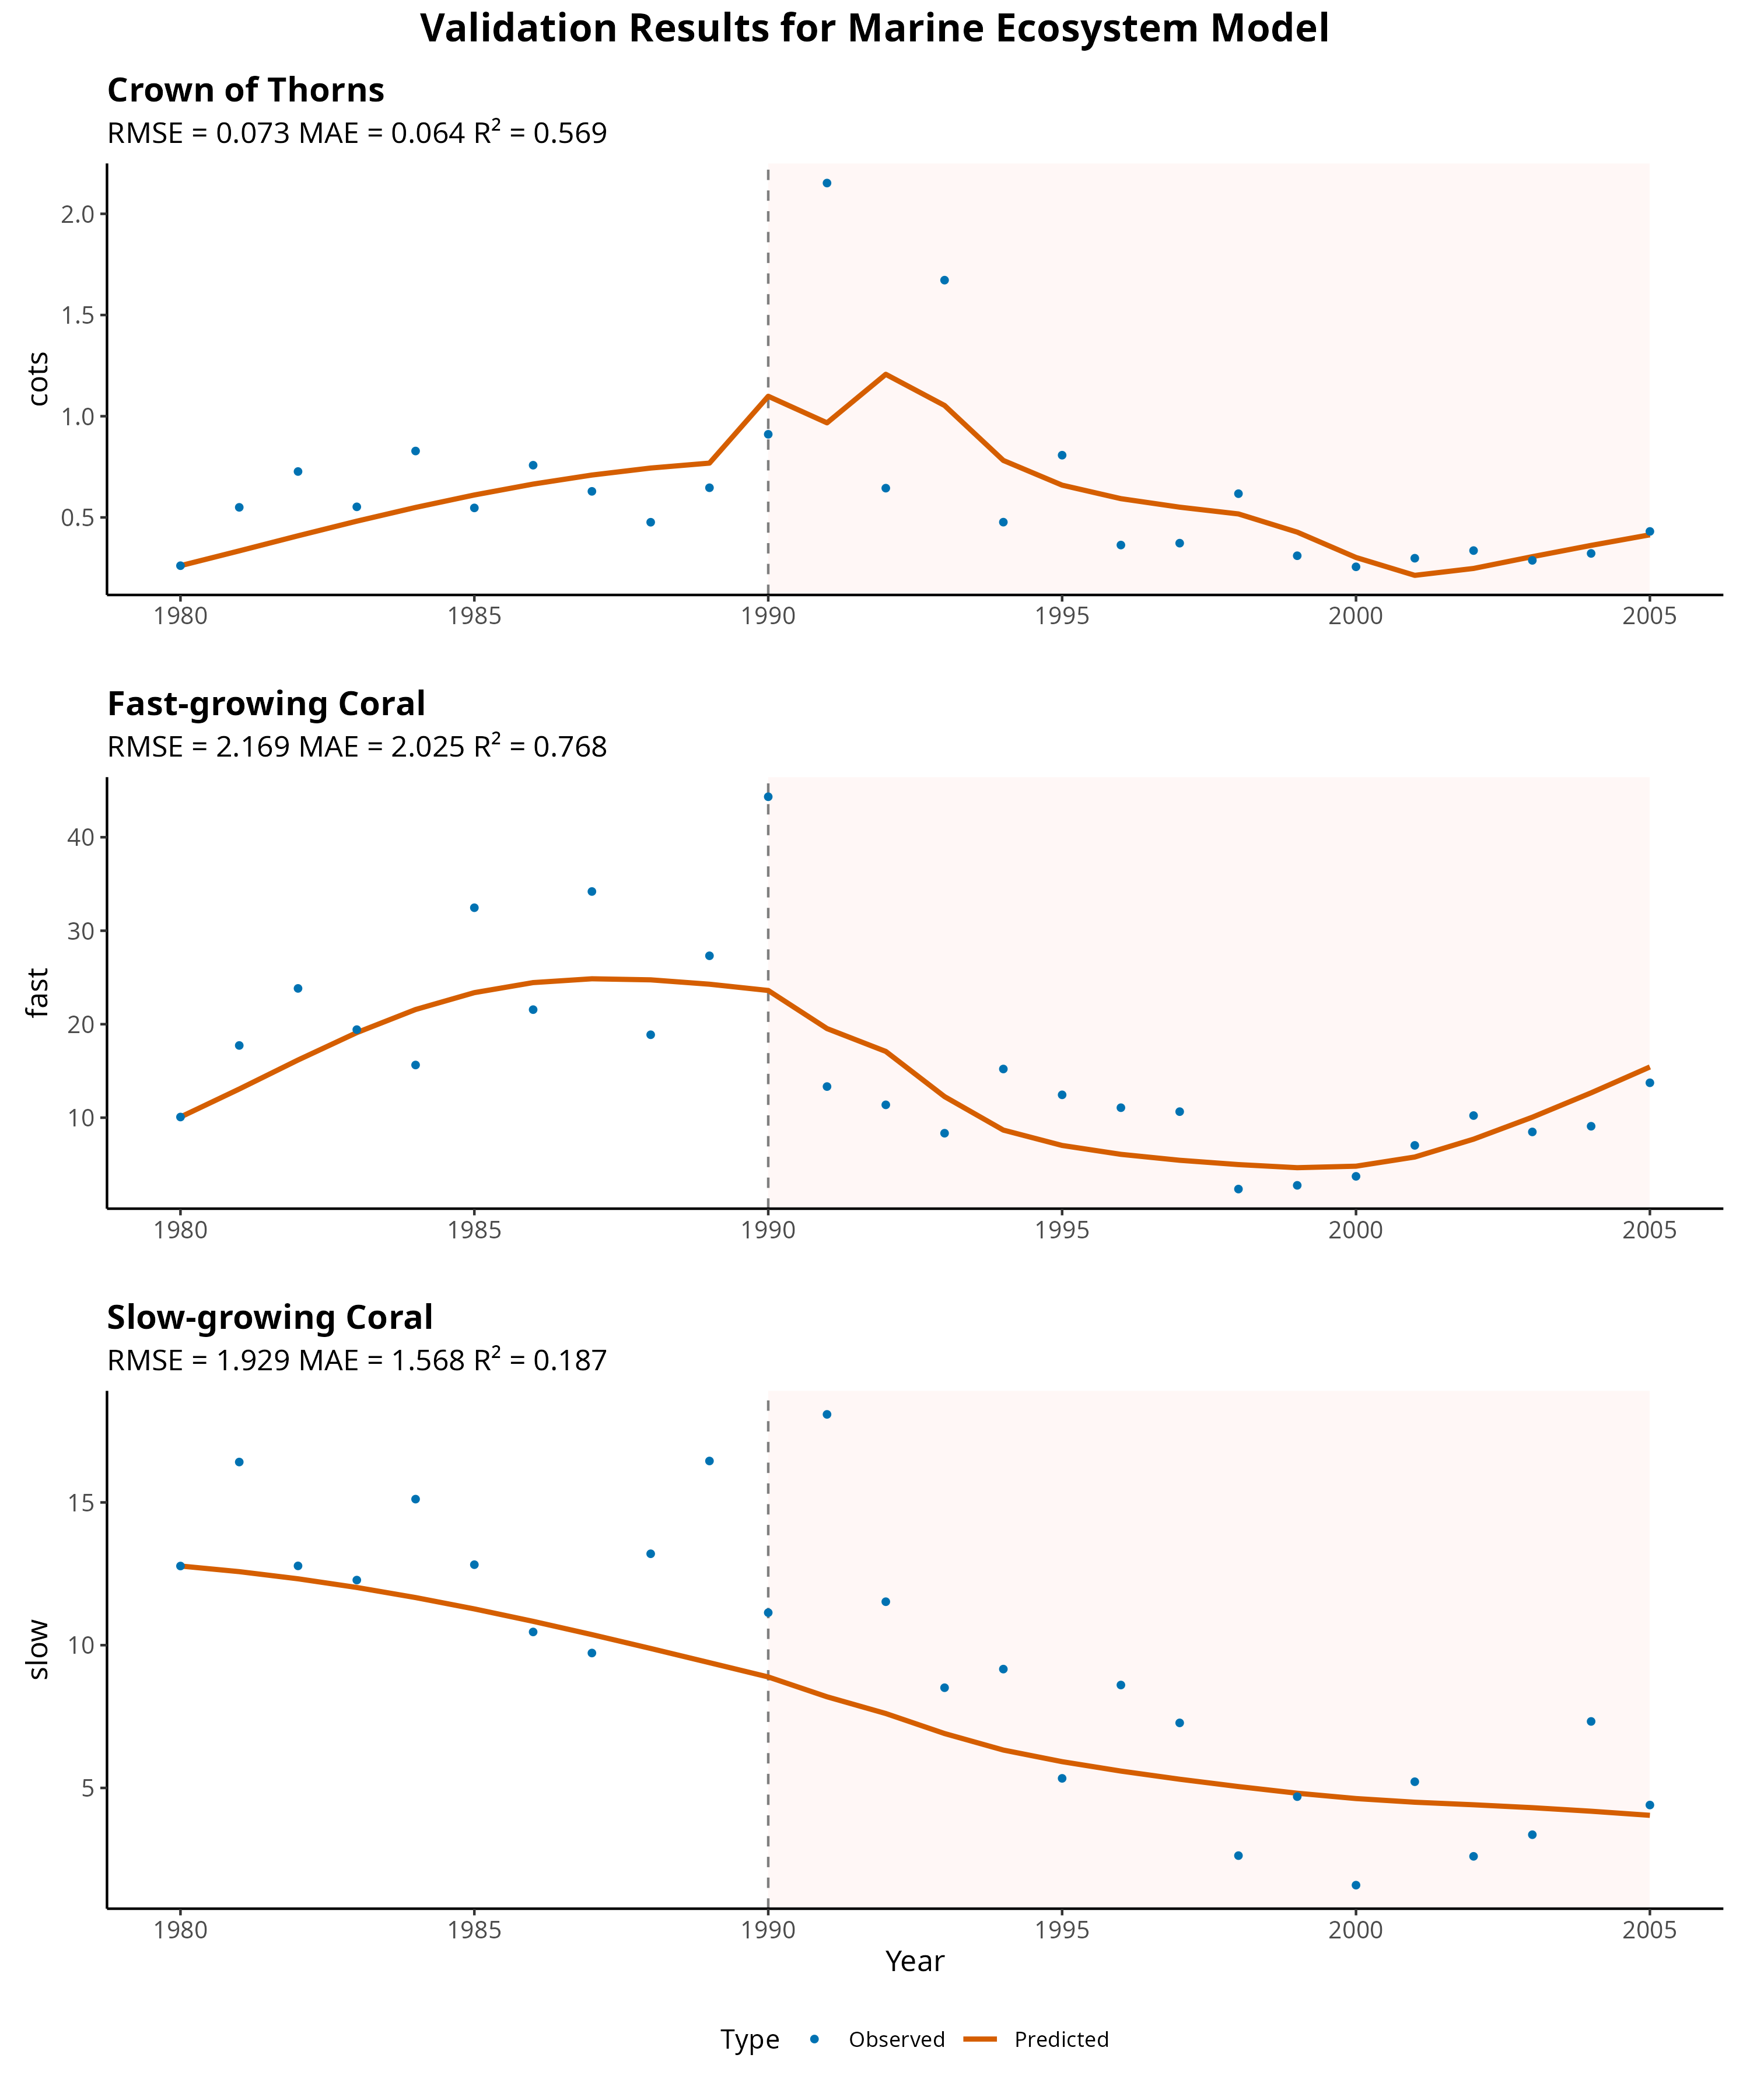
\includegraphics[width=1.0\textwidth]{../Figures/combined_validation.png}
\caption{Temporal hold-out evaluation of LEMMA driven by the best-performing LLM (GPT 4.1) showing predictions against observed data. LEMMA was provided with 70\% of the time-series data (pink shaded region) and developed a model that was then evaluated on the full time-series, including the remaining unseen 30\% of the time-series data (white region). Top: COTS abundance predictions showing some capture of population variability. Middle: Fast-growing coral cover predictions demonstrating tracking of recovering . Bottom: Slow-growing coral cover predictions illustrating strong capture of recovery dynamics. Orange lines represent model predictions, blue dots show observed data.}
\label{fig:validation_combined}
\end{figure}

\section{Discussion}
Our complementary validation studies demonstrate the viability of AI-driven automation in ecological model development and calibration. The NPZ validation revealed LEMMA's ability to recover known ecological relationships from synthetic data, with the best models achieving high ecological accuracy scores (up to 7.75 out of 8) while maintaining strong predictive performance (objective values as low as 0.112). While LEMMA did not perfectly reconstruct the original equations after 50 generations, it successfully identified key mechanisms like Michaelis-Menten kinetics and predator-prey interactions. The negative correlation between ecological accuracy and objective values suggests that improvements in model fit were achieved through discovery of correct ecological relationships rather than overfitting. This ability to balance model fit with ecological realism represents a significant advance in automated ecological modelling.

The CoTS case study further demonstrated LEMMA's practical utility, with LEMMA successfully generating models that approached the predictive performance of human expert models, albeit with less consistency across all variables. While the AI-derived models captured key ecological dynamics, they did so using structurally simpler formulations, and their performance varied depending on the specific ecosystem component being modeled.

Notably, the AI-generated models achieved predictive performance that was broadly similar to that of the human expert model, despite substantial structural differences. These results suggest that, under certain conditions, AI-driven approaches may approximate expert-level outcomes, though further validation and refinement are needed to ensure robustness and ecological fidelity (see Supplementary Materials for detailed comparison). While the human model implemented an age-structured COTS population with explicit age classes and a Beverton-Holt stock-recruitment relationship, the AI models generally employed simpler, unstructured population approaches. Similarly, the human model featured an explicit prey-switching function for COTS predation preference between coral types, whereas AI models used various functional responses ranging from coral-dependent reproduction to logistic growth with food limitation. These structural differences highlight an important trade-off: the human model exhibited greater mechanistic detail reflecting domain expertise and input from domain experts, while AI models achieved similar performance with more parsimonious formulations. This is consistent with the coexistence of multiple numerically valid representations of the same ecological system where each offers different insights into the underlying mechanisms \citep{patterson2001estimating}. 

Importantly, our findings also address the “forecast trap” described by \citep{Boettiger2022}, wherein selecting models primarily on predictive skill can lock decision-makers into policies that are accurate in forecast space but suboptimal in utility space. In capacity-constrained settings, having even a single model is often a luxury, and assembling an ensemble is typically out of reach. We hope that LEMMA, or tools like it, will enable diverse sets of models to be built, compared, and ensembled with relative ease. By evolving interpretable mechanistic candidates, LEMMA broadens the model set and supports robust decision workflows, reducing the risk of converging on a well-calibrated yet policy-misaligned model.

This flexibility also opens the door to hybrid approaches that combine the strengths of both expert-driven and AI-generated models. By explicitly prompting the AI to include particular ecological processes, such as age structure, prey-switching behavior, or nutrient mixing, researchers can guide model structure to reflect known system dynamics or stakeholder priorities. This capability enhances the utility of AI-generated models for hypothesis testing, scenario exploration, and applied decision-making, particularly in contexts where certain mechanisms are known to be ecologically or socially important. 

An important consideration in automated model generation is the provenance of parameter values. In this study, we restricted parameter retrieval to curated local literature and Semantic Scholar searches to ensure reliance on peer-reviewed information, noting that LEMMA incorporates the ability to also perform general web sources should the user choose. While restricting the source of parameter values improves transparency and scientific rigor, it also means that when literature values were unavailable, the system defaulted to LLM-derived initial estimates, which - though often plausible - lack explicit citation. Future enhancements such as user-defined whitelists and confidence scoring to further strengthen parameter provenance may help to address these limitations.

Unlike traditional machine-learning approaches which use regularisation and early-stopping to avoid overfitting. LEMMA employs two nested optimisation processes, both of may need mechanisms to address overfitting. For parameter estimation within TMB, literature-informed bounds act as weak regularisation, but no additional penalties are applied. For structural evolution, we limit changes to one modification per generation and cap the number of generations. In the NPZ case study, improvements in fit were negatively correlated with ecological accuracy scores, suggesting that gains were achieved through mechanistically sound changes rather than overfitting. Nonetheless, explicit complexity penalties or information-theoretic criteria (e.g., AIC/BIC) could further reduce overfitting risk in future iterations.

\subsection{Contrasting Approaches to AI in Ecological Modelling}
Recent advances in AI have demonstrated remarkable capabilities in ecological time-series prediction. Studies using transformer architectures and diffusion models, including multimodal approaches like LITE \citep{li2024lite}, have shown high accuracy in direct forecasting of environmental variables \citep{morales2024developing,gandhi2024generative}. While these methods effectively handle challenges like missing data and distribution shifts, they treat the system as a black box, learning patterns directly from time-series data without explicitly modelling underlying mechanisms. While our study did not directly compare our approach with black-box methods, our NPZ validation study suggests a key advantage of our approach: the ability to provide insights into fundamental ecological processes like nutrient cycling or predator-prey dynamics through explicit model discovery. This interpretability is a theoretical advantage over black-box approaches, though comparative studies would be needed to fully evaluate the relative strengths of each approach in specific ecological contexts.

Our evolutionary approach fundamentally differs by using AI to generate actual ecological models rather than make direct predictions. Instead of training neural networks to forecast future values, LEMMA evolves interpretable models with meaningful parameters that capture real biological and physical processes. This distinction is crucial for several reasons. First, our generated models provide scientific insight into system behavior, revealing mechanisms and relationships that direct prediction approaches typically cannot without careful oversight \citep{adams2017model}. Second, the models maintain biological plausibility through explicit parameter constraints and mechanistic formulations, ensuring their utility for management applications. Third, because they capture fundamental processes rather than just patterns, these models can potentially be transferred to new scenarios and used to explore management interventions.
The relationship between our approach and direct prediction methods is nuanced. Recent time-series prediction approaches using transformer architectures have achieved impressive accuracy, with mean squared errors as low as 0.001-0.04 for normalized predictions \citep{morales2024developing} and root mean squared errors reduced by up to 52\% compared to traditional methods \citep{gandhi2024generative}. While our evolved models may not always match these pure prediction accuracies, they offer advantages in interpretability, scientific insight and potential for strategic and tactical applications.

Importantly, these approaches need not be viewed as mutually exclusive. Comparing mechanistic models with black-box predictions can be particularly insightful, especially when the two approaches diverge. For instance, under novel conditions like future climate scenarios, differences in predictions could highlight processes that are not well-captured by mechanistic models or reveal patterns that black-box approaches detect but cannot explain. When predictive approaches outperform mechanistic models, this divergence can guide researchers toward missing processes or relationships that should be incorporated into mechanistic understanding. Our framework demonstrates that it's possible to achieve both reasonable predictive accuracy and meaningful ecological interpretability, with each approach offering complementary strengths.

This focus on model generation rather than direct prediction aligns with the needs of ecosystem-based management, where mechanistic understanding is as important as predictive accuracy. The interpretability of AI-evolved models enables users to assess the credibility of predictions and understand the mechanisms driving system behavior thereby allowing for informed management interventions, advantages not readily available with black-box prediction approaches. Work examining automated scientific discovery emphasizes the importance of maintaining human oversight while leveraging AI's computational capabilities \citep{kramer2023automated,Spillias2024}. Our approach directly addresses this need by producing interpretable models that facilitate meaningful human oversight while leveraging AI's capabilities for systematic exploration of model space. Crucially, this process is not solely computational: models are refined through expert collaboration, which synthesizes domain knowledge and builds confidence and legitimacy in the resulting models. This step is essential for filtering out plausible but ultimately incorrect mechanisms that may arise from AI-driven parsimony. For example, some temperature-related functions affecting COTS in the AI-derived models lack empirical support and thus their inclusion would likely be removed during expert-led refinement. While such mechanisms may be ecologically plausible, their inclusion without validation risks misleading management decisions, especially under extreme conditions. Thus, expert review acts as an important filter, ensuring that models are not only interpretable, but also credible and useful for decision-making.

\subsection{Limitations and Future Directions}

Despite promising results, several limitations warrant consideration. The observed variation in convergence rates across populations suggests that initial conditions significantly influence model evolution trajectories. While the best performing population achieved rapid convergence within five generations, other populations required more than twice as many generations to approach similar performance levels. In our current pipeline, convergence is also affected by the phased optimisation schedule and box-constraint handling: parameters are estimated in priority-ordered phases with starts clamped into literature- or LLM-derived bounds and pathological intervals normalised. Although these safeguards improve numerical stability, they can also interact with initial conditions in nontrivial ways (e.g., temporarily parking parameters on bound faces early in the schedule and delaying subsequent improvements).

An important limitation in our current implementation is the treatment of all model parameters as estimable quantities in the optimization process, even when well-established values exist in the literature. While our RAG system successfully retrieves some literature-based values and ranges for parameters, these are only used as initial estimates and bounds rather than as fixed quantities. This approach may lead to unnecessary parameter estimation and potential deviation from biologically meaningful values. Future versions of the framework should distinguish between parameters that truly need estimation and those that could be fixed based on reliable literature values. This would not only reduce the parameter space for optimization but also better incorporate established ecological knowledge into the modelling process and make the process less resource-intensive when doing calculations.

It is important to note that our prompt provided only high-level guidance on ecological realism, numerical stability, and reporting requirements, without specifying how parameter estimation should be implemented in TMB. Despite this minimal guidance, the LLM consistently generated models that adopt a forward-simulation approach: initializing at the first observation, simulating trajectories through time, and minimizing a trajectory-wide error metric. This convergence on a single strategy suggests that, under generic ecological modelling prompts, LLMs may default to conceptually straightforward but computationally fragile approaches. Future work could explore this outcome by explicitly prompting for alternative estimation paradigms, such as state-space formulations \citep{auger2021guide}, gradient matching \citep{ellner2002fitting}, or one-step-ahead prediction objectives \citep{munch2023recent}, thereby enabling systematic comparison of inference strategies within the same automated workflow.

There are numerous future avenues for validating, improving, and extending this framework. First, there are several hyper-parameters that likely control the success and speed of convergence of the framework (LLM-choice, LLM temperature setting, number of individuals per generation, prompt construction, etc.). Systematic testing across these choices may reveal optimal configurations for convergence. In particular, the comparative analysis of different AI configurations (as detailed in Section \ref{sec:cots_data} and Figure \ref{fig:status_distribution}) reveals trade-offs between model choice and rate of improvement. While the o3-mini and o4-mini configurations were consistently able to iteratively improve, the Sonnet models and GPT 4.1 model were often able to perform well in a single generation but then did not consistently improve. Future work could explore hybrid approaches that leverage the strengths of different AI configurations at various stages of model development, or that employ different LLMs consecutively over multiple generations. Further, ongoing testing of new LLMs as they are released may yield considerable gains in efficiency and cost-saving. Second, we have tested a relatively simple ecosystem model with three dependent variable time-series and two forcing variable time-series. Simple systems like these will be limited in real-world utility, and therefore testing on more complex systems with tens or hundreds of time-series will be needed. Incorporating spatial components may also be possible and will greatly improve the utility of this framework. Third, accessing relevant scientific information for the parameter RAG search is limited by the user's ability to either curate a local database of relevant materials, or access scientific papers online. Fourth, we have demonstrated that it is possible for this LLM-based system to generate multiple, distinct models for a given system. Choosing between similarly performing, but ecologically distinct models may be necessary for experts with ecological knowledge, or perhaps employing approaches that ensemble multiple plausible models may allow for the reduction in uncertainty \citep{baker2017ensemble,gaardmark2013biological,vollert2024unlocking}

\subsection{Implications for Ecosystem-Based Fisheries Management}

The successful application of LEMMA to COTS populations on the Great Barrier Reef demonstrates its potential for use in developing plausible models that can provie insights on pressing ecosystem problems relevant to ecosystem based management. While more development and experience is needed to ascertain AI-derived models directly into decision making contexts, there is certainly sufficient evidence that they can be used as a means of
hypothesis generation and for the development of plausible models. This may help to accelerate the model-building process, bringing the process more into line with timeframes pertinent to pressing tactical management questions. The framework's capacity to capture both short-term outbreak dynamics and longer-term ecosystem changes provides scientists supporting managers with valuable insights for intervention planning. The comparable performance between AI-generated models and human expert approaches suggests that automated modelling could complement traditional methods, accelerating the development and evaluation of management strategies.

While the current implementation of LEMMA demonstrates faster turnaround than typical manual workflows, reducing model development from weeks or months to hours, these gains reflect relatively simple case studies and yielded models of lesser complexity than human-generated models. As LEMMA matures and is tested in more complex systems, this enhanced efficiency may create capacity for more timely intervention in response to emerging ecological threats, such as in biosecurity emergencies, where management actions depend on rapid model development and deployment. LEMMA's ability to integrate multiple data sources, both locally and from web search, and account for both biological and environmental factors provides a robust foundation for developing early warning systems and evaluating potential management interventions.\

\begin{figure}[htbp]
    \centering
    \includegraphics[width=\textwidth]{../Figures/AIME_workflow.drawio.png}
    \caption{The LEMMA framework workflow integrating human expertise with AI-driven model development. The diagram illustrates how stakeholder engagement, time-series data, and prior ecological knowledge inform the LEMMA process, which generates candidate models that can be evaluated and refined by human experts, ultimately supporting ecosystem management decisions.}
    \label{fig:aime_workflow}
\end{figure}


To ensure safe and effective integration of LEMMA into ecosystem-based fisheries management, we recommend a set of best practices and propose that LEMMA would work best embedded within a human-driven workflow (Figure \ref{fig:aime_workflow}). 

\begin{enumerate}
    \item \textbf{Stakeholder Engagement}  
    Begin with stakeholder engagement to inform problem framing and define the ecological questions LEMMA will address. Early involvement ensures models are relevant to management needs and incorporate local knowledge.

    \item \textbf{Expert Review}  
    All AI-generated models should be reviewed by domain experts to validate ecological plausibility and ensure alignment with management objectives.

    \item \textbf{Complementary Use}  
    Use LEMMA as a complementary tool that supports - rather than replaces - traditional modelling workflows, especially for rapid prototyping or exploring alternative hypotheses.

    \item \textbf{Model Transparency}  
    Maintain transparency through clear documentation of equations, parameters, and assumptions to ensure traceability and reproducibility.

    \item \textbf{Parameter Assessment}  
    Critically assess parameter values sourced from literature. Fix well-established values where appropriate to reduce uncertainty.

    \item \textbf{Rigorous Validation}  
    Conduct thorough validation, including cross-validation and out-of-sample testing, before applying models to decision-making.

    \item \textbf{Training and Capacity Building}  
    Provide training to ensure managers and researchers can interpret and apply AI-generated models responsibly.
\end{enumerate}

In conclusion, LEMMA represents an advancement in ecological modelling that bridges the gap between computational efficiency and ecological insight. By dramatically accelerating model development while maintaining scientific rigour, this framework offers a powerful new tool for researchers and managers facing urgent ecological challenges. As environmental pressures intensify globally, the capacity to rapidly develop, test, and deploy ecologically sound models will become increasingly valuable for effective conservation and management of marine ecosystems.



% Backmatter sections for the manuscript

\section*{Acknowledgements}
SS was supported by an R+ Postdoctoral Fellowship. 

\section*{Code and Data Availability}
The code for the AIME framework is available in a public GitHub repository at \url{https://github.com/s-spillias/EMs-with-LLMs}. The repository includes all scripts necessary to reproduce the results presented in this paper, including the genetic algorithm implementation, model evaluation tools, and analysis scripts. The time series data used in the case studies are also available in the repository. The software is released under an MIT license.

\section*{Declaration on Generative AI Usage}
During the preparation of this manuscript, we used Claude-3.5-Sonnet, a large language model, to assist with code documentation, manuscript formatting, and language editing. The scientific content, analyses, interpretations, and conclusions presented in this paper were developed and validated by the human authors. 

\section*{Author Contributions}
SS: Conceptualization, Methodology, Software, Data curation, Formal analysis, Writing - original draft, Writing - review \& editing
JR: Software, Methodology, Data curation, Writing - review \& editing
FB: Formal analysis, Supervision, Writing - review \& editing
BF: Formal analysis, Supervision, Writing - review \& editing
RT: Supervision, Writing - review \& editing
MG: Software, Methodology, Writing - review \& editing
SY: Software, Methodology, Writing - review \& editing

\section*{Competing Interests}
The authors declare no competing interests.

\section*{Data Availability}
The datasets generated and analyzed during the current study are available in the GitHub repository \url{https://github.com/s-spillias/EMs-with-LLMs}. Additional data that support the findings of this study are available from the corresponding author upon reasonable request.



\bibliographystyle{apalike}
\bibliography{references}

\clearpage
\appendix
\clearpage
\section*{Supplementary Information: An AI-Driven Framework for Automated Generation of Marine Ecosystem Models}

\setcounter{section}{0}
\renewcommand{\thesection}{S\arabic{section}}

\section{Curated Literature Collection}
\label{subsec:curated_literature}

The local document collection used in this case study was carefully curated to provide comprehensive coverage of marine ecosystem modeling approaches, with particular focus on COTS-coral dynamics and management interventions. The collection encompasses several key research areas:

\begin{itemize}
\item Ecosystem Modeling Frameworks: \cite{Plaganyi_2007} established foundational principles for ecosystem approaches to fisheries, while \cite{Plaganyi_Punt_Hillary_Morello_Thebaud_Hutton_Pillans_Thorson_Fulton_Smith_et_al_2014} introduced Models of Intermediate Complexity for Ecosystem assessments (MICE). \cite{Collie_Botsford_Hastings_Kaplan_Largier_Livingston_Plaganyi_Rose_Wells_Werner_2016} explored optimal model complexity levels.

\item COTS Management and Ecology: \cite{Pratchett_Caballes_Wilmes_Matthews_Mellin_Sweatman_Nadler_Brodie_Thompson_Hoey_et_al_2017} provided a comprehensive thirty-year review of COTS research. \cite{morello2014model} developed models for COTS outbreak management, while \cite{Rogers_Plaganyi_2022} analyzed corallivore culling impacts under bleaching scenarios.

\item Ecological Regime Shifts: \cite{Blamey_Plaganyi_Branch_2014} investigated predator-driven regime shifts in marine ecosystems. \cite{Plaganyi_Ellis_Blamey_Morello_Norman-Lopez_Robinson_Sporcic_Sweatman_2014} provided insights into ecological tipping points through ecosystem modeling.

\item Management Interventions: \cite{Condie_Anthony_Babcock_Baird_Beeden_Fletcher_Gorton_Harrison_Hobday_Plaganyi_et_al_2021} examined large-scale interventions on the Great Barrier Reef. \cite{Punt_MacCall_Essington_Francis_Hurtado-Ferro_Johnson_Kaplan_Koehn_Levin_Sydeman_2016} explored harvest control implications using MICE models.

\item Model Application Guidelines: \cite{Essington_Plaganyi_2014} provided critical guidelines for adapting ecosystem models to new applications. \cite{Gamble_Link_2009} demonstrated multispecies production model applications for analyzing ecological and fishing effects.

\item Integrated Systems: \cite{Hadley_Wild-Allen_Johnson_Macleod_2015} and \cite{Oca_Cremades_Jimenez_Pintado_Masalo_2019} explored integrated multi-trophic aquaculture modeling, providing insights into coupled biological systems. \cite{Spillias_Cottrell_2024} analyzed trade-offs in seaweed farming between food production, livelihoods, marine biodiversity, and carbon sequestration benefits.
\end{itemize}

These papers were selected based on their direct relevance to COTS population dynamics, coral reef ecology, and ecosystem modeling approaches. The collection provided both specific parameter values and broader ecological context for model development.

\section{RAG Architecture Implementation}
\label{subsec:rag_architecture}

The Retrieval-Augmented Generation (RAG) system facilitates parameter search and extraction from scientific literature. The system employs two primary search strategies: a local search of user-curated documents and a comprehensive web search. For local search, the system uses ChromaDB as a persistent vector store to maintain an indexed collection of scientific papers and technical documents specifically curated by research teams for their ecological systems. These documents are processed into semantic chunks of approximately 512 tokens with small overlaps to preserve context while enabling precise retrieval of relevant information.

The parameter search process begins with the generation of enhanced semantic descriptions for each parameter. These descriptions are crafted to improve search relevance by capturing the ecological and mathematical context in which the parameters are used. The system first searches the user-curated local documents using embeddings generated through Azure OpenAI's embedding service. When necessary, it extends to web-based sources through two channels: querying the Semantic Scholar database for highly-cited papers in biology, mathematics, and environmental science, and conducting broader literature searches through the Serper API to capture additional relevant sources.

The search results from both local and web sources are processed through an LLM to extract numerical values. The system applies consistent validation across both search pathways, identifying minimum and maximum bounds, ensuring unit consistency, and validating source reliability. When direct parameter values are not found in either the local collection or web sources, the system defaults to the initial estimates from the coding LLM. All extracted information, including parameter values, valid ranges, and complete citation details, is stored in a structured JSON database for reproducibility and future reference.

The RAG system implements automatic retry mechanisms when initial searches fail to yield usable results. Each retry attempt follows a structured progression: first accessing the curated local collection through ChromaDB queries, then expanding to Semantic Scholar for peer-reviewed literature, and finally utilizing Serper API for broader scientific content. This progressive broadening of scope, while maintaining focus on ecologically relevant sources, ensures robust parameter estimation even in cases where direct measurements are sparse in the literature.

\section{AI Prompts Used in Model Development}
\label{sec:ai_prompts}

The development of the model relied on several carefully crafted prompts to guide the artificial intelligence system. These prompts were designed to ensure numerical stability, proper likelihood calculation, and clear model structure. The following sections detail the exact prompts used at each stage of model development.

\subsection{Initial Model Creation}
\label{subsec:initial_model_prompt}

The initial model creation utilized a comprehensive prompt that emphasized three key aspects of model development. The prompt used for model initialization was:

\begin{lstlisting}
Please create a Template Model Builder model for the following topic:[PROJECT_TOPIC]. Start by writing intention.txt, in which you provide a concise summary of the ecological functioning of the model. In model.cpp, write your TMB model with the following important considerations:

1. NUMERICAL STABILITY:
- Always use small constants (e.g., Type(1e-8)) to prevent division by zero
- Use smooth transitions instead of hard cutoffs in equations
- Bound parameters within biologically meaningful ranges using smooth penalties rather than hard constraints

2. LIKELIHOOD CALCULATION:
- Always include observations in the likelihood calculation, don't skip any based on conditions
- Use fixed minimum standard deviations to prevent numerical issues when data values are small
- Consider log-transforming data if it spans multiple orders of magnitude
- Use appropriate error distributions (e.g., lognormal for strictly positive data)

3. MODEL STRUCTURE:
- Include comments after each line explaining the parameters (including their units and how to determine their values)
- Provide a numbered list of descriptions for the equations
- Ensure all important variables are included in the reporting section
- Use `_pred' suffix for model predictions corresponding to `_dat' observations
\end{lstlisting}

\subsection{Parameter Enhancement}
\label{subsec:parameter_enhancement_prompt}

To enhance parameter descriptions for improved semantic search capabilities, the following prompt was employed:

\begin{lstlisting}
Given a mathematical model about [PROJECT_TOPIC], enhance the semantic descriptions of these parameters to be more detailed and searchable. The model code shows these parameters are used in the following way:

[MODEL_CONTENT]

For each parameter below, create an enhanced semantic search, no longer than 10 words, that can be used for RAG search or semantic scholar search.
\end{lstlisting}

\subsection{Model Improvement}
\label{subsec:model_improvement_prompt}

For iterative model improvements, the system utilized this prompt:

\begin{lstlisting}
Improve the fit of the following ecological model by modifying the equations in this TMB script. Only make ONE discrete change most likely to improve the fit. Do not add stochasticity, but you may add other ecological relevant factors that may not be present here already.

You may add additional parameters if necessary, and if so, add them to parameters.json. Please concisely describe your ecological improvement in intention.txt and then provide the improved model.cpp and parameters.json content.

\end{lstlisting}

\subsection{Error Handling Prompts}
\label{subsec:error_handling_prompt}

For compilation errors, the system used this prompt:

\begin{lstlisting}
model.cpp failed to compile. Here's the error information:

[ERROR_INFO]

Do not suggest how to compile the script
\end{lstlisting}

For data leakage issues, the system employed this detailed prompt:

\begin{lstlisting}
Data leakage detected in model equations. The following response variables cannot be used to predict themselves:

To fix this:
1. Response variables ([RESPONSE_VARS]) must be predicted using only:
   - External forcing variables ([FORCING_VARS])
   - Other response variables' predictions (_pred variables)
   - Parameters and constants
2. Each response variable must have a corresponding prediction equation
3. Use ecological relationships to determine how variables affect each other

For example, instead of:
  slow_pred(i) = slow * growth_rate;
Use:
  slow_pred(i) = slow_pred(i-1) * growth_rate * (1 - impact_rate * cots_pred(i-1));

Please revise the model equations to avoid using response variables to predict themselves.
\end{lstlisting}

For numerical instabilities, the system used an adaptive prompt that became progressively more focused on simplification after multiple attempts:

\begin{lstlisting}
The model compiled but numerical instabilities occurred. Here's the error information:

[ERROR_INFO]

[After 2+ attempts: Consider making a much simpler model that we can iteratively improve later.]
Do not suggest how to compile the script
\end{lstlisting}

\subsection{NPZ Case Study - Recovering Equations}
\label{subsec:npz_evaluation_prompt}

The model implementation can be compared to the original NPZ equations from \cite{edwards1999zooplankton}:

\begin{align*}
    \frac{dN}{dt} &= \underbrace{-\frac{V_m N P}{k_s + N}}_{\text{nutrient uptake}}
                   + \underbrace{\gamma(1-\alpha)\frac{g P^2 Z}{k_g + P^2} + \mu_P P + \mu_Z Z^2}_{\text{recycling}}
                   + \underbrace{S(N_0 - N)}_{\text{mixing}} \\[6pt]
    \frac{dP}{dt} &= \underbrace{\frac{V_m N P}{k_s + N}}_{\text{growth}}
                   - \underbrace{\frac{g P^2 Z}{k_g + P^2}}_{\text{grazing loss}}
                   - \underbrace{\mu_P P}_{\text{mortality}}
                   - \underbrace{S P}_{\text{mixing}} \\[6pt]
    \frac{dZ}{dt} &= \underbrace{\alpha\frac{g P^2 Z}{k_g + P^2}}_{\text{growth (assimilation)}}
                   - \underbrace{\mu_Z Z^2}_{\text{mortality}}
                   - \underbrace{S Z}_{\text{mixing}}
    \end{align*}

Our generated model captures several key ecological processes from the original system:
\begin{enumerate}
\item Nutrient uptake by phytoplankton following Michaelis-Menten kinetics
\item Quadratic zooplankton mortality
\item Nutrient recycling through zooplankton excretion
\item Environmental mixing effects
\end{enumerate}

For evaluating the ecological characteristics of generated models against the NPZ reference model, the system employed a 4-level ordinal scoring system that compares each model component to both the ground truth equations and recognized alternate formulations from the ecological literature. The evaluation system assessed nine ecological characteristics organized by equation: nutrient uptake, recycling, and mixing (dN/dt); phytoplankton growth, grazing loss, mortality, and mixing (dP/dt); and zooplankton growth and mortality (dZ/dt).

The scoring rubric used for all evaluations was:

\begin{lstlisting}
Scoring rubric per characteristic (choose exactly one category):
- 3 = TRUTH_MATCH
    The mathematical structure is equivalent to the TRUTH model (modulo variable names,
    syntax, factor grouping, and coefficient naming). Quote the exact snippet that matches.
- 2 = ALTERNATE
    The implementation matches one of the alternates enumerated in the literature catalog,
    even if not identical to TRUTH. Name the family (e.g., "Michaelis-Menten uptake",
    "Ivlev grazing with threshold", "linear mortality", "Droop quota").
- 1 = SIMILAR_NOT_LISTED
    The implementation plays the same ecological role and is mathematically similar
    (e.g., another saturating curve or plausible closure) but is not represented in TRUTH
    or alternates list.
- 0 = NOT_PRESENT_OR_INCORRECT
    The ecological component is missing or cannot be identified.
\end{lstlisting}

The alternate formulations catalog was based on \cite{franks2002npz} and included:

\begin{itemize}
    \item Phytoplankton light response: linear, saturating (Michaelis-Menten, exponential, tanh), and photo-inhibiting forms
    \item Nutrient uptake: Michaelis-Menten, Liebig minimum limitation, Droop quota models
    \item Zooplankton grazing: linear, saturating with threshold, Holling/Ivlev type, acclimating forms
    \item Mortality terms: linear and quadratic (density-dependent) for both phytoplankton and zooplankton
\end{itemize}

Each characteristic was assigned a weight based on its contribution to its parent equation: the three nutrient equation components each had weight 0.333, the four phytoplankton components each had weight 0.25, and the two zooplankton components each had weight 0.5. The aggregate ecological score was calculated as the weighted sum of individual scores, then normalized to a 0-1 scale by dividing by the maximum possible score.

\subsubsection{Validation of Scoring System}

To validate the ecological characteristics scoring system, we tested it on the ground truth NPZ model itself (evaluating the model against its own equations). This test confirmed that the scoring system could correctly identify and score all nine ecological characteristics when they were present in their canonical forms.

The validation results demonstrated perfect performance:

\begin{itemize}
    \item All nine characteristics received scores of 3 (TRUTH\_MATCH)
    \item Raw total score: 8.997 (out of maximum 9.0, with small rounding due to floating point arithmetic)
    \item Normalized total score: 1.0000 (perfect score on 0-1 scale)
    \item Zero extra components identified (correctly recognized model contained only canonical NPZ processes)
\end{itemize}

The LLM evaluator correctly identified each ecological mechanism in the ground truth model, providing detailed explanations such as ``algebraically identical to the TRUTH NPZ model'' and specifically noting the presence of ``Michaelis-Menten style nutrient limitation multiplied by a light/self-shading term for phytoplankton growth'' and ``a saturating P\textsuperscript{2}/(µ\textsuperscript{2}+P\textsuperscript{2}) (Hill/Type-III-like) grazing formulation.'' This validation confirmed that the scoring system could reliably distinguish between different levels of ecological fidelity, from exact matches to the ground truth through recognized alternates to novel formulations, providing a robust framework for assessing LEMMA-generated models.

\section{NPZ Validation}
\label{sec:npz_validation}

\subsection{Best Performing NPZ Model}

\subsubsection{Model Description}
The following model represents our framework's attempt to recover the NPZ dynamics from \cite{edwards1999zooplankton}. The model aims to capture three key components:
\begin{itemize}
\item Nutrient uptake and recycling
\item Phytoplankton growth and mortality
\item Zooplankton predation and dynamics
\end{itemize}

\subsubsection{Model Intention}
\begin{lstlisting}
\section{Ecological Intention}

A key modification was made to incorporate direct nutrient recycling from zooplankton grazing activity. In marine systems, zooplankton feeding is often inefficient, with a significant portion of consumed phytoplankton being released as dissolved nutrients rather than being assimilated into biomass or entering the detritus pool. This "sloppy feeding" process creates an important feedback loop where grazing can stimulate new primary production through rapid nutrient recycling.

The recycling efficiency is temperature-dependent, reflecting how metabolic rates and feeding mechanics vary with temperature. This creates an adaptive feedback where warmer conditions lead to both increased grazing pressure and faster nutrient recycling, better capturing the coupled nature of predator-prey interactions in planktonic systems.

The modification introduces a direct pathway from grazing to dissolved nutrients, complementing the slower recycling through the detritus pool. This better represents the multiple timescales of nutrient cycling in marine food webs and helps explain how high productivity can be maintained even under intense grazing pressure.
\end{lstlisting}

\subsubsection{Model Implementation}
\newpage
\section*{NPZ Model: Parameter and Equation Tables}

\begin{landscape}
\subsection*{Parameter summary}

\begin{table}[ht]
\centering
\scriptsize
\setlength{\tabcolsep}{4pt}
\begin{tabular}{l p{3cm} p{10cm} c l l l}
\toprule
Symbol & Units & Meaning & Init.\ value & Bounds & Source & Literature (citekey) \\
\midrule
log\_mu\_max & day$^{-1}$ (log scale) & Log of maximum phytoplankton growth rate at reference conditions (day$^{-1}$). & -0.02 & [-0.22, 0.18] & literature & Yes (LitNPZ\_log\_mu\_max) \\
log\_K\_N & g C m$^{-3}$ (log scale) & Log of half-saturation constant for nutrient uptake (g C m$^{-3}$). & -3.00 & [-6.91, 0.00] & literature & Yes (LitNPZ\_log\_K\_N) \\
I & W m$^{-2}$ & Mean photosynthetically active irradiance proxy over the modeled period. & 150.00 & [0.00, 500.00] & initial estimate & No \\
log\_K\_I & W m$^{-2}$ (log scale) & Log of light half-saturation constant for photosynthesis (W m$^{-2}$). & 4.32 & [0.00, 5.70] & literature & Yes (LitNPZ\_log\_K\_I) \\
log\_g\_max & day$^{-1}$ (log scale) & Log of maximum zooplankton grazing rate per unit Z biomass (day$^{-1}$). & -0.69 & [-3.00, 0.69] & literature & Yes (LitNPZ\_log\_g\_max) \\
log\_K\_G & g C m$^{-3}$ (log scale) & Log of P half-saturation constant for grazing functional response (g C m$^{-3}$). & -2.30 & [-6.91, 0.00] & literature & Yes (LitNPZ\_log\_K\_G) \\
h\_grazing & dimensionless & Holling type III shape exponent (h $\ge$ 1). & 2.00 & [1.00, 3.00] & literature & Yes (LitNPZ\_h\_grazing) \\
logit\_e\_Z & dimensionless (logit scale) & Logit of zooplankton assimilation efficiency ($e_Z \in (0,1)$); $e_Z = 0.5$ at value 0. & 0.00 & \textemdash & literature & Yes (LitNPZ\_logit\_e\_Z) \\
log\_m\_P & day$^{-1}$ (log scale) & Log of phytoplankton linear mortality rate (day$^{-1}$). & -3.00 & [-6.91, -1.20] & literature & Yes (LitNPZ\_log\_m\_P) \\
log\_m\_Z & day$^{-1}$ (log scale) & Log of zooplankton linear mortality rate (day$^{-1}$). & -3.51 & [-6.91, -1.20] & literature & Yes (LitNPZ\_log\_m\_Z) \\
log\_gamma\_Z & (g C m$^{-3}$)$^{-1}$ day$^{-1}$ (log scale) & Log of zooplankton quadratic self-limitation coefficient ((g C m$^{-3}$)$^{-1}$ day$^{-1}$). & -4.61 & [-9.21, -1.61] & initial estimate & No \\
logit\_r\_P & dimensionless (logit scale) & Logit of fraction of P mortality that is remineralized to N (0..1). & 0.85 & \textemdash & literature & Yes (LitNPZ\_logit\_r\_P) \\
logit\_r\_Z & dimensionless (logit scale) & Logit of fraction of Z mortality that is remineralized to N (0..1). & 0.85 & \textemdash & literature & Yes (LitNPZ\_logit\_r\_Z) \\
log\_ex\_Z & day$^{-1}$ (log scale) & Log of zooplankton excretion rate to nutrients (day$^{-1}$). & -4.61 & [-13.82, -1.61] & initial estimate & No \\
log\_k\_mix & day$^{-1}$ (log scale) & Log of vertical mixing rate driving nutrients toward $N_\star$ (day$^{-1}$). & -3.91 & [-13.82, -0.69] & initial estimate & No \\
$N_\star$ & g C m$^{-3}$ & Deep/source nutrient concentration towards which mixing relaxes the system. & 0.30 & [0.00, 2.00] & initial estimate & No \\
log\_q10 & dimensionless (log scale) & Log of Q10 temperature scaling factor (dimensionless), typical $Q10 \approx 2$. & 0.66 & [0.61, 0.71] & literature & Yes (LitNPZ\_log\_q10) \\
T\_C & deg C & Ambient temperature used for Q10 scaling (deg C). & 15.00 & [0.00, 35.00] & initial estimate & No \\
T\_ref & deg C & Reference temperature for Q10 scaling (deg C). & 15.00 & [0.00, 35.00] & literature & Yes (LitNPZ\_T\_ref) \\
log\_k\_rem & day$^{-1}$ (log scale) & Log of detritus remineralization rate to nutrients (day$^{-1}$). & -2.30 & [-4.61, 0.00] & conceptual addition & No \\
log\_k\_sink & day$^{-1}$ (log scale) & Log of detritus sinking/export rate out of mixed layer (day$^{-1}$). & -4.61 & [-13.82, 0.00] & conceptual addition & No \\
log\_sigma\_N & log-scale SD & Log of observation SD for N on the log scale. & -2.30 & [-5.00, 2.00] & initial estimate & No \\
log\_sigma\_P & log-scale SD & Log of observation SD for P on the log scale. & -2.30 & [-5.00, 2.00] & initial estimate & No \\
log\_sigma\_Z & log-scale SD & Log of observation SD for Z on the log scale. & -2.30 & [-5.00, 2.00] & initial estimate & No \\
\bottomrule
\end{tabular}
\end{table}

\end{landscape}

\section{CoTS Model Convergence}
\label{sec:convergence}
    
\subsection{Model Evolution and Convergence}
The evolutionary process exhibited consistent refinement across generations, with measurable improvements in model performance. On average, populations reached their best-performing individual within 6.9 generations, and the mean improvement frequency across all populations was 38.0\%. Figure \ref{fig:status_distribution} shows the distribution of successful, culled, and broken models across generations. Notably, two populations achieved convergence below the target threshold, representing 9.5\% of all populations.
Performance varied significantly across populations. The fastest-converging population reached an optimal objective value of 0.0035 in just 3 generations, while others required up to 13 generations. This population also demonstrated a high improvement rate of -0.655 and a consistent improvement frequency of 50\%. In contrast, several populations showed minimal or no improvement, with some failing to converge within the allotted iterations.
\begin{figure}[H]
\centering
\includegraphics[width=0.8\textwidth]{../Figures/success_frequency}
\caption{Evolution of model performance during the genetic algorithm optimization process. Each generation represents an iteration of model development, where models are evaluated and classified into three categories: the best performers according to the NMSE objective value (kept, green), those that are numerically stable but outcompeted (culled, blue), and those that failed due to numerical instability, data leakage, or syntax errors (broken, orange). The vertical axis shows the count of new models in each category per generation, while rows represent independent replicates using different LLM configurations. Gemini-2.5-Pro was included in the analysis but did not produce successful runs for some populations.}
\label{fig:status_distribution}
\end{figure}

\subsection{Numerical Stability and Optimization}
Numerical stability varied across LLM configurations, with runtime and generation time metrics reflecting differences in optimization efficiency. The GPT-5 configuration showed moderate efficiency, with an average generation time of 12.0 minutes (SD = 13.0). The Claude Sonnet 4.5 configuration had longer generation times, averaging 71.2 minutes (SD = 155.2), though this includes variability from a small number of outlier populations. In contrast, the Gemini-2.5-Pro configuration demonstrated the fastest generation cycles, averaging 4.1 minutes per generation (SD = 0.54), though it exhibited lower convergence rates and higher instability in some cases.
Figure \ref{fig:iterations_by_llm} illustrates the distribution of iteration counts required for successful model convergence across LLMs. Most models converged within 4 to 7 iterations, with some outliers requiring up to 11 iterations.
\begin{figure}[H]
\centering
\includegraphics[width=0.8\textwidth]{../Figures/iterations_by_llm}
\caption{Distribution of iteration counts for successful model instances by LLM configuration. The boxplot excludes cases that reached maximum iterations or remained numerically unstable.}
\label{fig:iterations_by_llm}
\end{figure}


\section{Comparative Analysis of Best-Performing Models}
\label{sec:model_comparison}

Before presenting the full code for each model, we analyze the key differences between the best-performing models to understand their ecological approaches and mathematical structures.

% 
\subsection{Key Parameter Comparison}
\label{subsec:parameter_comparison}

Table \ref{tab:parameter_comparison} presents a detailed comparison of key parameters across the five best-performing models and the human-generated model. These parameters represent fundamental ecological processes and reveal different modelling approaches to COTS-coral dynamics.

\begin{landscape}
\begin{table}[H]
\centering
\begin{footnotesize}
\caption{Comparison of key parameters across best-performing models}
\label{tab:parameter_comparison}
\begin{tabular}{p{3.2cm}p{2.8cm}p{2.8cm}p{2.8cm}p{2.8cm}p{2.8cm}p{2.8cm}}
 
\textbf{Parameter} & \textbf{Human Model} & \textbf{o3 mini} & \textbf{Claude Sonnet 3.6} & \textbf{Claude Sonnet 3.7} & \textbf{o4 mini} & \textbf{gpt 4.1} \\
 
COTS growth rate (yr$^{-1}$) & Beverton-Holt (h=0.5) & exp(log\_growth\_rate) & 0.8 & 0.8 & 0.5 & 0.5 \\
 
COTS mortality (yr$^{-1}$) & Mcots = 2.3 & exp(log\_decline\_rate) & -- & 0.4 & 0.3 & 0.37 \\
 
COTS carrying capacity & Derived from R0=1.0 & -- & 2.0 & 2.5 & 50 & 0.61 \\
 
Slow coral growth (yr$^{-1}$) & rm = 0.1 & 0.1 (fixed) & 0.2 & 0.1 & 0.05 (fixed) & 0.37 \\
 
Fast coral growth (yr$^{-1}$) & rf = 0.5 & 0.2 (fixed) & 0.4 & 0.3 & 0.1 (fixed) & 0.61 \\
 
Coral carrying capacity & K = 3000 (shared) & -- & 0.8 & K\_slow = 30, K\_fast = 50 & -- & K\_slow = 20.1, K\_fast = 33.1 \\
 
Fast coral optimal temp (°C) & SST0\_f = 26 & -- & -- & -- & -- & -- \\
 
Slow coral optimal temp (°C) & SST0\_m = 27 & -- & -- & -- & -- & -- \\
 
COTS optimal temp (°C) & Implicit & -- & 28 & 28 & -- & -- \\
 
Attack rate (fast coral) & p1f = 0.15 & 0.4 & 0.1 & 0.2 & 0.05 & 0.14 \\
 
Attack rate (slow coral) & p1m = 0.06 & 0.6 & 0.05 & 0.05 & 0.05 & 0.08 \\
 
Predation switching & switchSlope = 5 & -- & -- & -- & -- & -- \\
 
Functional response & Sigmoid switching & Logistic with quadratic adjustment & Type II & Type II & Type III & Type II \\
 
\end{tabular}
\end{footnotesize}
\end{table}
\end{landscape}

\subsection{Model Structure Comparison}
\label{subsec:structure_comparison}

Table \ref{tab:equation_comparison} presents a detailed comparison of the key equations used in each model, highlighting the different mathematical approaches to representing COTS-coral dynamics.


\begin{longtable}{p{2cm}p{13cm}}
\caption{Comparison of key equations across models}\label{tab:equation_comparison} \\

\textbf{Model} & \textbf{Key Equations} \\
 
\endfirsthead

\multicolumn{2}{c}%
{{\bfseries \tablename\ \thetable{} -- continued from previous page}} \\

\textbf{Model} & \textbf{Key Equations} \\
 
\endhead

\multicolumn{2}{r}{{Continued on next page}} \\
\endfoot


\endlastfoot
Human Model &
\begin{tabular}[t]{p{12.5cm}}
\textbf{COTS dynamics:} \\
Age-structured model with three age classes (0, 1, 2+) \\
$N(yr+1,1) = N(yr,0) \cdot \exp(-1 \cdot M\_CoTS\_age(0))$ \\
$N(yr+1,2) = N(yr,1) \cdot \exp(-f \cdot M\_CoTS\_age(1)) + N(yr,2) \cdot \exp(-f \cdot M\_CoTS\_age(2))$ \\
$Rcots(yr+1) = \frac{\alpha \cdot (N(yr+1,2)/Kots\_sp)}{\beta + (N(yr+1,2)/Kots\_sp)}$ \\
$N(yr+1,0) = (Rcots(yr+1) + Imm\_CoTS) \cdot \exp(Imm\_res(yr+1) + \sigma_{CoTS}^2/2)$ \\
\\
\textbf{Coral dynamics:} \\
$Cf(yr+1) = Cf(yr) \cdot (1.0 + \rho_{SST\_F} \cdot rf \cdot (1-(Cf(yr) + Cm(yr))/K)) - Qf - M\_ble\_f$ \\
$Cm(yr+1) = Cm(yr) \cdot (1.0 + \rho_{SST\_M} \cdot rm \cdot (1-(Cf(yr) + Cm(yr))/K)) - Qm - M\_ble\_m$ \\
\\
\textbf{Predation:} \\
$\rho = \exp(-switchSlope \cdot Cf(yr)/K)$ \\
$Qf = Cf(yr) \cdot (1.0-\rho) \cdot p1f \cdot \frac{N(yr,1)+N(yr,2)}{1.0+\exp(-(N(yr,1)+N(yr,2))/p2f)}$ \\
$Qm = Cm(yr) \cdot \rho \cdot p1m \cdot \frac{N(yr,1)+N(yr,2)}{1.0+\exp(-(N(yr,1)+N(yr,2))/p2m)}$ \\
\\
\textbf{Temperature effects:} \\
$\rho_{SST\_F} = \exp(-\frac{(SST-SST0\_f)^2}{2 \cdot SST\_sig\_f^2})$ \\
$\rho_{SST\_M} = \exp(-\frac{(SST-SST0\_m)^2}{2 \cdot SST\_sig\_m^2})$ \\
$M\_ble\_f = Cf(yr) \cdot \frac{1.0}{1.0 + \exp(-Eta\_f \cdot (SST-M\_SST50\_f))}$ \\
$M\_ble\_m = Cm(yr) \cdot \frac{1.0}{1.0 + \exp(-Eta\_m \cdot (SST-M\_SST50\_m))}$
\end{tabular} \\
 
o3 mini &
\begin{tabular}[t]{p{12.5cm}}
\textbf{COTS dynamics:} \\
$logistic\_factor = \frac{1}{1 + \exp(-outbreak\_steepness \cdot (resource\_limitation - threshold))}$ \\
$quadratic\_adjustment = \begin{cases}
1 + poly\_coeff \cdot (resource\_limitation - threshold)^2 & \text{if } resource\_limitation > threshold \\
1 & \text{otherwise}
\end{cases}$ \\
$outbreak\_factor = logistic\_factor \cdot quadratic\_adjustment$ \\
$temperature\_factor = 1 + effect\_sst \cdot sst\_dat(t-1)$ \\
$cots\_pred[t] = cots\_pred[t-1] + (growth\_rate \cdot cots\_pred[t-1] \cdot outbreak\_factor \cdot temperature\_factor - decline\_rate \cdot cots\_pred[t-1]) \cdot dt$ \\
\\
\textbf{Coral dynamics:} \\
$fast\_pred[t] = fast\_pred[t-1] + dt \cdot (fast\_growth\_rate \cdot fast\_pred[t-1] \cdot (1 - fast\_pred[t-1] / fast\_cap) - efficiency\_fast \cdot cots\_pred[t-1] \cdot fast\_pred[t-1])$ \\
$mod\_eff\_slow = efficiency\_slow \cdot (1 + temp\_mod\_eff\_slow \cdot sst\_dat(t-1))$ \\
$slow\_pred[t] = slow\_pred[t-1] + dt \cdot (slow\_growth\_rate \cdot slow\_pred[t-1] \cdot (1 - slow\_pred[t-1] / slow\_cap) - mod\_eff\_slow \cdot cots\_pred[t-1] \cdot slow\_pred[t-1])$
\end{tabular} \\
 
Claude Sonnet 3.6 &
\begin{tabular}[t]{p{12.5cm}}
\textbf{COTS dynamics:} \\
$temp\_effect = \exp(-0.5 \cdot \frac{(sst\_dat(t-1) - temp\_opt)^2}{temp\_range^2})$ \\
$resource\_limit = \frac{total\_coral}{total\_coral + \epsilon}$ \\
$recruitment = cotsimm\_dat(t-1) \cdot temp\_effect$ \\
$cots\_pred(t) = cots\_pred(t-1) \cdot (1 + r\_cots \cdot resource\_limit \cdot (1 - \frac{cots\_pred(t-1)}{K\_cots})) + recruitment$ \\
\\
\textbf{Coral dynamics:} \\
$coral\_space = \max(0, 1 - \frac{fast\_pred(t-1) + slow\_pred(t-1)}{100 \cdot coral\_limit})$ \\
$fast\_growth = r\_fast \cdot fast\_pred(t-1) \cdot coral\_space$ \\
$fast\_pred\_loss = grazing\_fast \cdot cots\_pred(t-1) \cdot fast\_pred(t-1)$ \\
$fast\_pred(t) = fast\_pred(t-1) + fast\_growth - fast\_pred\_loss$ \\
$slow\_growth = r\_slow \cdot slow\_pred(t-1) \cdot coral\_space$ \\
$slow\_pred\_loss = grazing\_slow \cdot cots\_pred(t-1) \cdot slow\_pred(t-1)$ \\
$slow\_pred(t) = slow\_pred(t-1) + slow\_growth - slow\_pred\_loss$
\end{tabular} \\
 
Claude Sonnet 3.7 &
\begin{tabular}[t]{p{12.5cm}}
\textbf{COTS dynamics:} \\
$temp\_effect = \exp(-0.5 \cdot \frac{(sst - temp\_opt)^2}{temp\_width^2})$ \\
$pred\_fast = \frac{a\_fast \cdot fast\_t0 \cdot cots\_t0}{1.0 + a\_fast \cdot h\_fast \cdot fast\_t0 + a\_slow \cdot h\_slow \cdot slow\_t0 + \epsilon}$ \\
$pred\_slow = \frac{a\_slow \cdot slow\_t0 \cdot cots\_t0}{1.0 + a\_fast \cdot h\_fast \cdot fast\_t0 + a\_slow \cdot h\_slow \cdot slow\_t0 + \epsilon}$ \\
$bleach\_effect = \frac{1.0}{1.0 + \exp(-2.0 \cdot (sst - bleach\_threshold))}$ \\
$cots\_growth = r\_cots \cdot cots\_t0 \cdot (1.0 - \frac{cots\_t0}{K\_cots}) \cdot temp\_effect$ \\
$imm\_term = \frac{imm\_effect \cdot cotsimm}{1.0 + cotsimm + \epsilon}$ \\
$food\_limitation = m\_cots \cdot (1.0 + \frac{1.0}{fast\_t0 + slow\_t0 + \epsilon})$ \\
$cots\_pred(t) = cots\_t0 + cots\_growth - food\_limitation \cdot cots\_t0 + imm\_term$ \\
\\
\textbf{Coral dynamics:} \\
$fast\_growth = r\_fast \cdot fast\_t0 \cdot (1.0 - \frac{fast\_t0 + competition \cdot slow\_t0}{K\_fast})$ \\
$fast\_bleaching = bleach\_mortality\_fast \cdot bleach\_effect \cdot fast\_t0$ \\
$fast\_pred(t) = fast\_t0 + fast\_growth - pred\_fast - fast\_bleaching$ \\
$slow\_growth = r\_slow \cdot slow\_t0 \cdot (1.0 - \frac{slow\_t0 + competition \cdot fast\_t0}{K\_slow})$ \\
$slow\_bleaching = bleach\_mortality\_slow \cdot bleach\_effect \cdot slow\_t0$ \\
$slow\_pred(t) = slow\_t0 + slow\_growth - pred\_slow - slow\_bleaching$
\end{tabular} \\
 
o4 mini &
\begin{tabular}[t]{p{12.5cm}}
\textbf{COTS dynamics:} \\
$coral\_availability = \frac{fast\_pred[t-1] + slow\_pred[t-1]}{200}$ \\
$resource\_factor = \frac{coral\_availability + coral\_saturation\_coefficient \cdot coral\_availability^2}{0.5 + coral\_availability + coral\_saturation\_coefficient \cdot coral\_availability^2}$ \\
$growth = growth\_rate\_cots \cdot cots\_pred[t-1] \cdot (1 - \frac{cots\_pred[t-1]}{carrying\_capacity + \epsilon}) \cdot (1 + resource\_limitation\_strength \cdot (resource\_factor - 0.5))$ \\
$effective\_sharpness = outbreak\_sharpness \cdot environmental\_modifier \cdot (1 + extreme\_outbreak\_modifier \cdot (environmental\_modifier - 1))$ \\
$raw\_trigger = \frac{1}{1 + \exp(- effective\_sharpness \cdot (cots\_pred[t-1]^{outbreak\_shape} + outbreak\_nonlinearity \cdot cots\_pred[t-1]^2 - (outbreak\_threshold \cdot carrying\_capacity)^{outbreak\_shape}))}$ \\
$outbreak\_trigger = raw\_trigger + outbreak\_hysteresis \cdot raw\_trigger \cdot (1 - raw\_trigger)$ \\
$decline = decay\_rate\_cots \cdot cots\_pred[t-1]^{outbreak\_decline\_exponent} \cdot outbreak\_trigger$ \\
$cots\_pred[t] = cots\_pred[t-1] + growth - decline$ \\
\\
\textbf{Coral dynamics:} \\
$fast\_pred[t] = fast\_pred[t-1] + 0.1 \cdot coral\_recovery\_modifier \cdot coral\_recovery\_environmental\_modifier \cdot (100 - fast\_pred[t-1]) \cdot (1 - coral\_recovery\_inhibition \cdot \frac{cots\_pred[t-1]}{carrying\_capacity + \epsilon}) - \frac{cots\_pred[t-1] \cdot coral\_predation\_efficiency \cdot fast\_pred[t-1] \cdot (\frac{fast\_pred[t-1]}{fast\_pred[t-1] + predation\_scaler})^{predation\_efficiency\_exponent}}{1 + handling\_time \cdot fast\_pred[t-1]}$ \\
$slow\_pred[t] = slow\_pred[t-1] + 0.05 \cdot coral\_recovery\_environmental\_modifier \cdot (100 - slow\_pred[t-1]) \cdot (1 - coral\_recovery\_inhibition \cdot \frac{cots\_pred[t-1]}{carrying\_capacity + \epsilon}) - \frac{cots\_pred[t-1] \cdot coral\_predation\_efficiency \cdot slow\_pred[t-1] \cdot (\frac{slow\_pred[t-1]}{slow\_pred[t-1] + predation\_scaler})^{predation\_efficiency\_exponent}}{1 + handling\_time \cdot slow\_pred[t-1]}$
\end{tabular} \\

gpt 4.1 &
\begin{tabular}[t]{p{12.5cm}}
\textbf{COTS dynamics:} \\
$coral\_effect = \frac{fast\_prev \cdot e\_fast + slow\_prev \cdot e\_slow}{K\_fast \cdot e\_fast + K\_slow \cdot e\_slow + \epsilon}$ \\
$sst\_effect = 1.0 + theta\_sst \cdot (sst\_dat(t) - 27.0)$ \\
$immig\_effect = immig\_scale \cdot cotsimm\_dat(t)$ \\
$outbreak\_boost = 1.0 + phi\_outbreak \cdot (coral\_effect - 0.5)$ \\
$cots\_growth = r\_cots \cdot cots\_prev \cdot (1.0 - \frac{cots\_prev}{K\_cots + \epsilon}) \cdot coral\_effect \cdot sst\_effect \cdot outbreak\_boost$ \\
$cots\_mortality = m\_cots \cdot cots\_prev$ \\
$cots\_next = cots\_prev + cots\_growth - cots\_mortality + immig\_effect$ \\
\\
\textbf{Coral dynamics:} \\
$pred\_fast = \frac{\alpha\_fast \cdot cots\_prev \cdot fast\_prev}{fast\_prev + slow\_prev + \epsilon}$ \\
$pred\_slow = \frac{\alpha\_slow \cdot cots\_prev \cdot slow\_prev}{fast\_prev + slow\_prev + \epsilon}$ \\
$fast\_growth = r\_fast \cdot fast\_prev \cdot (1.0 - \frac{fast\_prev}{K\_fast + \epsilon})$ \\
$fast\_mortality = m\_fast \cdot fast\_prev$ \\
$fast\_next = fast\_prev + fast\_growth - pred\_fast - fast\_mortality$ \\
$slow\_growth = r\_slow \cdot slow\_prev \cdot (1.0 - \frac{slow\_prev}{K\_slow + \epsilon})$ \\
$slow\_mortality = m\_slow \cdot slow\_prev$ \\
$slow\_next = slow\_prev + slow\_growth - pred\_slow - slow\_mortality$
\end{tabular}
\end{longtable}

\subsection{Detailed Ecological Mechanisms}
\label{subsec:ecological_mechanisms}
\begin{landscape}
\begin{table}[htbp]
\centering
\footnotesize
\setlength{\tabcolsep}{3pt}
\renewcommand{\arraystretch}{1.2}
\begin{tabularx}{\linewidth}{@{}lXXXX@{}}
\toprule
\textbf{Mechanism (anchored to Human \texttt{CoTSmodel\_v4.cpp})} &
\textbf{Human v4} &
\textbf{Google Gemini 2.5 Pro} &
\textbf{OpenAI GPT--5} &
\textbf{Anthropic Claude Sonnet 4.5} \\
\midrule
\textbf{COTS state structure / life history} &
\textit{Age-structured (3 classes)}: \(N_{t+1,1} = N_{t,0} e^{-M_0}\); \(N_{t+1,2} = N_{t,1} e^{-f M_1} + N_{t,2} e^{-f M_2}\); recruits form \(N_{t+1,0}\). Age-specific mortality \(M_a = M_{\text{cots}} + \lambda /(1+a)\). &
\textit{Single compartment} \(C_t\) (no explicit ages). Growth from consumption + modifiers. &
\textit{Two-stage} (juveniles \(J\) and adults \(C\)): maturation \(m_J J\); juvenile mortality \(\mu_J J\); adult mortality \((\mu_C + \gamma_C C)C\). &
\textit{Single compartment} with logistic-like adult growth plus additive recruitment pulse; no age classes. \\
\midrule
\textbf{COTS stock--recruitment} &
\textit{Beverton--Holt (BH) from spawners}:
\(R_{t+1} = \dfrac{\alpha (N_{t+1,2}/K_{\text{sp}})}{\beta + (N_{t+1,2}/K_{\text{sp}})}\),
with \(\alpha,\beta\) derived from slope steepness \(h\) and \(R_0\). &
\textit{Not BH}:
recruitment implicit via \(\big(e_F \cdot \text{Cons}_F + e_S \cdot \text{Cons}_S\big)\)
\(\times\) Allee \(\times\) temperature Gaussian (no explicit SR function). &
\textit{BH-like taper on adults}:
\(\text{Rec} = \alpha_{\text{rec}}\,[ C^\phi /(1 + C/C_{\text{sat}} ) ] \cdot f_{\text{Allee}}(C) \cdot f_T(\text{SST}) \cdot f_{\text{food}}
+ \text{imm}_{t-1}\). &
\textit{Additive pulse recruitment}:
\(\text{recruit\_pulse} = R_{\max}\cdot \sigma\!\big(\text{fav}-\tau\big)\cdot \text{fav}\),
added to adult change; adult growth also logistic-like. \\
\midrule
\textbf{COTS immigration \& interannual pulses} &
\textit{Background immigration} + year-specific deviations:
\(N_{t+1,0} = (R_{t+1} + \text{Imm}_{\text{CoTS}})\exp(\varepsilon_{t+1} + \sigma^2/2)\);
\(\varepsilon_t\) applied in specified years. &
Exogenous additive series \(\text{cotsimm}(t)\) added directly to \(C_t\) dynamics. &
Exogenous series \(\text{cotsimm}_{t-1}\) added to recruitment (lagged). &
Used twice:
(i) normalized within favorability index, and
(ii) multiplicative \(\text{immigration\_boost} = 1 + \text{effect}\cdot \text{imm}\) on adult growth. \\
\midrule
\textbf{COTS mortality and its drivers} &
\textit{Baseline + age-dependent}, modulated by coral availability:
effective multiplier \(f = (1 - \tilde p) + \tilde p \cdot \rho\) (see prey switching \(\rho\));
applied to age-1 and age-2+ mortality; mortality reduced when fast coral abundant. &
\textit{No age structure};
mortality = survival Allee
\(\dfrac{m_{C,\max} C}{1 + C/A_{\text{mort}}}\)
\(+\) quadratic density dependence \(m_{C,\text{dd}} C^2\);
not explicitly coral-modulated. &
\textit{No age structure};
adult mortality \((\mu_C + \gamma_C C) C\);
not explicitly coral-modulated. &
\textit{No age structure};
baseline + density-dependent mortality,
\textbf{amplified by starvation}:
multiplier \(1 + 2\,e^{- (F+S)/5}\) increases mortality when coral scarce. \\
\midrule
\textbf{Prey switching / diet preference} &
\textit{Abundance-driven switching}:
\(\rho = \exp(-\text{switchSlope}\cdot F/K)\).
Predation share on fast coral \(\propto (1-\rho)\), on slow \(\propto \rho\).
As fast coral increases, switch toward fast prey. &
Implicit via multi-prey Type II with separate \(a_F, a_S\); no explicit \(\rho\) rule. &
Implicit via Type II/III blend (exponents \(\eta_F,\eta_S\) create low-prey refuge); no explicit \(\rho\). &
\textit{Preference + availability}:
weight combines fixed preference with fast-coral proportion (soft switching toward abundant prey). \\
\midrule
\textbf{Functional response (COTS $\rightarrow$ coral consumption)} &
\textit{Sigmoid-saturated vs COTS density}:
\(Q_F = F\,(1-\rho)\,p_{1F}\,\dfrac{N_{1+2}}{1+\exp\!\big(-N_{1+2}/p_{2F}\big)}\),
\(Q_M = S\,\rho\,p_{1M}\,\dfrac{N_{1+2}}{1+\exp\!\big(-N_{1+2}/p_{2M}\big)}\). &
\textit{Multi-prey Holling Type II}:
per-capita
\(\dfrac{a_F F}{1 + a_F h F + a_S h S}\),
\(\dfrac{a_S S}{1 + a_F h F + a_S h S}\);
totals scale with \(C\). &
\textit{Type II/III blend}:
\(\text{Cons}_F = q_F \dfrac{a_F F^{\eta_F} C}{1 + h(a_F F^{\eta_F} + a_S S^{\eta_S})}\),
\(\text{Cons}_S = q_S \dfrac{a_S S^{\eta_S} C}{1 + h(a_F F^{\eta_F} + a_S S^{\eta_S})}\). &
\textit{Type II per prey} with separate handling;
then \textit{preference weighting} mixes fast vs slow consumption. \\
\midrule
\textbf{Coral intrinsic growth \& space competition} &
\textit{Logistic regrowth with shared space}:
\(\displaystyle F_{t+1} = F_t \Big[1 + \rho_F(\text{SST})\, r_f \Big(1 - \tfrac{F_t + S_t}{K}\Big)\Big] - Q_F - M_{\text{ble},F}\);
analogous for \(S\). &
\textit{Logistic regrowth} with shared \(K_{\text{coral}}\);
losses: predation + bleaching mortality. &
\textit{Logistic regrowth} with shared \(K_{\text{tot}}\);
losses: predation + heat-related terms. &
\textit{Logistic regrowth} with shared \(K_{\text{coral}}\);
losses: predation + temperature-stress mortality. \\
\midrule
\textbf{SST modulation of coral regrowth (performance curve)} &
\textit{Gaussian performance multiplier}:
\(\rho_F(\text{SST}) = \exp\!\left[-\dfrac{(\text{SST} - \text{SST0}_f)^2}{2\,\text{SST\_sig}_f^2}\right]\),
\(\rho_M(\text{SST}) = \exp\!\left[-\dfrac{(\text{SST} - \text{SST0}_m)^2}{2\,\text{SST\_sig}_m^2}\right]\). &
Not Gaussian on growth; SST enters via \textit{logistic bleaching mortality} (see below). &
\textit{Heat-stress growth reduction}:
multiplier \(\exp[-\beta_{\text{bleach}} \max(0, \text{SST} - T_{\text{bleach}})]\) on growth (non-Gaussian). &
\textit{Threshold stress loss}:
linear mortality above \(T_{\text{stress}}\); no Gaussian growth multiplier. \\
\midrule
\textbf{Coral bleaching mortality} &
\textit{Logistic bleaching}:
\(M_{\text{ble},F} = F \cdot \big[1 + \exp\{-\eta_f(\text{SST} - M_{50,F})\}\big]^{-1}\);
analogous for slow coral (impulse option commented). &
\textit{Logistic bleaching mortality}:
\(m_{F,\text{sst}} / \big[1 + \exp\{-k_{\text{bleach}}(\text{SST} - T_{\text{bleach},F})\}\big]\);
applied proportionally to \(F\); analogous for \(S\). &
Two components:
(i) multiplicative \textit{growth reduction} under heat,
(ii) \textit{additional linear loss} \(m_{\text{bleach}} \cdot \text{heat} \cdot \text{coral}\);
no logistic 50\% curve. &
\textit{Temperature-stress mortality} proportional to degrees above threshold;
no explicit logistic bleaching curve. \\
\midrule
\textbf{Coral carrying capacity (space sharing)} &
\textit{Shared \(K\)} via \(1 - (F+S)/K\) in both coral equations. &
\textit{Shared \(K_{\text{coral}}\)} in coral logistic growth. &
\textit{Shared \(K_{\text{tot}}\)} in coral logistic growth. &
\textit{Shared \(K_{\text{coral}}\)} in coral logistic growth. \\
\bottomrule
\end{tabularx}
\caption{Side-by-side comparison of ecological mechanisms and mathematical implementations across the human-generated reference model (\texttt{CoTSmodel\_v4.cpp}) and three LLM-generated models. The rows are anchored to mechanisms explicitly present in the human model; each LLM implementation is summarized without parameter values. Symbols: \(C\) adult COTS, \(J\) juvenile COTS, \(F,S\) fast/slow coral cover, \(K\) shared coral carrying capacity, \(\text{SST}\) sea surface temperature.}
\label{tab:mechanism_comparison}
\end{table}
\end{landscape}

\begin{landscape}
\begin{table}[htbp]
\centering
\footnotesize
\renewcommand{\arraystretch}{1.15}
\setlength{\tabcolsep}{3pt}
\begin{tabularx}{\linewidth}{@{}l l l l X@{}}
\toprule
\textbf{Human (name)} & \textbf{Role / Units} & \textbf{Gemini 2.5 Pro} & \textbf{OpenAI GPT--5} & \textbf{Claude Sonnet 4.5} \\
\midrule
\texttt{Mcots} & Baseline instantaneous COTS mortality (yr$^{-1}$) &
$m_{C,\max}$ (low-density mortality scale); $m_{C,\text{dd}}$ (DD mortality) &
$\mu_C$ (baseline adult mortality), $\gamma_C$ (DD mortality) &
$\texttt{log\_mort\_base}$ (baseline), $\texttt{log\_mort\_density}$ (DD) \\
\texttt{lam} & Age-dependence of mortality, $M_a = M_{\rm cots}+\lambda/(1+a)$ &
--- (no age structure) & --- (two-stage but no age-specific $M$) & --- (no age structure) \\
\texttt{ptil} & Fraction of $M$ attributable to fast-coral availability (mortality modulation) &
--- (no coral-modulated $M$) &
--- (no coral-modulated $M$) &
Starvation multiplier $1+2e^{-(F+S)/5}$ (different form) \\
\texttt{h} (BH steepness) & Shapes SR via $(R_0,h)\rightarrow \alpha,\beta$ &
--- (no BH SR; growth from consumption) &
$C_{\text{sat,rec}}$ (BH-like taper), $\alpha_{\rm rec}$, $\phi$ (fecundity exponent) &
Recruitment pulse parameters: $\texttt{log\_recruit\_max}$, $\texttt{recruit\_threshold}$ \\
\texttt{R0} & Recruitment at unexploited state (for SR derivation) &
--- (no explicit $R_0$) &
$\alpha_{\rm rec}$ (scales juvenile input; closest analogue) &
$\texttt{log\_recruit\_max}$ (caps pulse magnitude; different structure) \\
\texttt{Imm\_CoTS} & Background immigration (ind m$^{-2}$ yr$^{-1}$) &
$\texttt{cotsimm\_dat}(t)$ (added to adults each step) &
$\texttt{cotsimm\_dat}(t\!-\!1)$ (added into recruitment) &
$\texttt{cotsimm\_dat}$ used in favorability and as growth boost \\
\texttt{sigCoTS} & SR process variability (lognormal on recruits) &
--- (no process noise term; observation SD only) &
--- (no explicit process noise on SR; observation SDs) &
--- (no explicit process noise on SR; observation SDs) \\
\texttt{immigration} & Year-specific recruitment deviations (vector by year) &
Represent via time series in $\texttt{cotsimm\_dat}$ &
Represent via time series in $\texttt{cotsimm\_dat}$ &
Represent via time series in $\texttt{cotsimm\_dat}$ \\
\texttt{COTS\_init} & Initial COTS abundance (age-2+) &
Init from first data row (no param) &
$C0$ (adults), $J0$ (juveniles) &
Init from first data row (no param) \\
\bottomrule
\end{tabularx}
\caption{COTS demography and recruitment parameter mapping. Human model uses age classes and Beverton--Holt SR; Gemini uses consumption-driven growth; GPT--5 uses BH-like SR on adults with environmental modifiers; Claude adds an episodic recruitment pulse.}
\label{tab:params_cots}
\end{table}
\end{landscape}

\begin{landscape}
\begin{table}[htbp]
\centering
\footnotesize
\renewcommand{\arraystretch}{1.15}
\setlength{\tabcolsep}{3pt}
\begin{tabularx}{\linewidth}{@{}l l l l X@{}}
\toprule
\textbf{Human (name)} & \textbf{Role / Units} & \textbf{Gemini 2.5 Pro} & \textbf{OpenAI GPT--5} & \textbf{Claude Sonnet 4.5} \\
\midrule
\texttt{p1f}, \texttt{p1m} & Per-COTS coral loss coefficients (fast/slow), units of \% cover $\cdot$ (ind$^{-1}$ yr$^{-1}$) &
$a_F,a_S$ (attack), $h$ (handling) with efficiencies $e_F,e_S$ for COTS growth (coral loss $\propto$ consumption) &
$aF,aS$ (attack), $h$ (handling), $qF,qS$ (loss efficiencies) \quad(Type II/III via $\eta_F,\eta_S$) &
$\texttt{log\_attack\_fast/slow}$, $\texttt{log\_handling\_fast/slow}$, plus preference weighting \\
\texttt{p2f}, \texttt{p2m} & Logistic saturation vs COTS density (shape of $Q_F,Q_M$) &
Denominator $1+a_FhF+a_ShS$ (resource-based saturation; no explicit p2) &
Denominator $1+h(a_FF^{\eta_F}+a_SS^{\eta_S})$ (no explicit p2) &
Separate Type-II denominators per prey (no explicit p2) \\
\texttt{switchSlope} & Controls prey switching: $\rho=\exp(-\text{switchSlope}\cdot F/K)$ &
--- (no explicit $\rho$) &
$\eta_F,\eta_S$ (Type-III curvature; soft switching), no $\rho$ &
$\texttt{preference\_fast}$ blended with fast-coral share (soft switching) \\
\bottomrule
\end{tabularx}
\caption{Predation and prey-switching parameters. Human model uses COTS-density logistic saturation (via $p2$) and an explicit exponential switching function; LLMs use Holling multi-prey forms with handling and (in GPT--5) Type-III exponents; Claude adds an explicit preference term.}
\label{tab:params_predation}
\end{table}
\end{landscape}

\begin{landscape}
\begin{table}[htbp]
\centering
\footnotesize
\renewcommand{\arraystretch}{1.15}
\setlength{\tabcolsep}{3pt}
\begin{tabularx}{\linewidth}{@{}l l l l X@{}}
\toprule
\textbf{Human (name)} & \textbf{Role / Units} & \textbf{Gemini 2.5 Pro} & \textbf{OpenAI GPT--5} & \textbf{Claude Sonnet 4.5} \\
\midrule
\texttt{K} & Shared coral carrying capacity (\% cover scale) &
$K_{\text{coral}}$ (\texttt{log\_K\_coral} parameterized) &
$K_{\text{tot}}$ &
$K_{\text{coral}}$ (\texttt{log\_K\_coral}) \\
\texttt{rf}, \texttt{rm} & Intrinsic regrowth (fast/slow), yr$^{-1}$ &
$r_F,r_S$ (\texttt{log\_r\_F}, \texttt{log\_r\_S}) &
$rF,rS$ &
$r_{\text{fast}},r_{\text{slow}}$ (\texttt{log\_r\_fast}, \texttt{log\_r\_slow}) \\
\texttt{Cf\_init}, \texttt{Cm\_init} & Initial coral state (fraction of $K$) &
Init from first data row (no param) &
$F0,S0$ &
Init from first data row (no param) \\
\bottomrule
\end{tabularx}
\caption{Coral demography and space limitation. All models use a shared carrying capacity for two coral groups; GPT--5 exposes explicit initial-state parameters.}
\label{tab:params_coral}
\end{table}
\end{landscape}

\begin{landscape}
\begin{table}[htbp]
\centering
\footnotesize
\renewcommand{\arraystretch}{1.15}
\setlength{\tabcolsep}{3pt}
\begin{tabularx}{\linewidth}{@{}l l l l X@{}}
\toprule
\textbf{Human (name)} & \textbf{Role / Units} & \textbf{Gemini 2.5 Pro} & \textbf{OpenAI GPT--5} & \textbf{Claude Sonnet 4.5} \\
\midrule
\texttt{Eta\_f}, \texttt{Eta\_m} & Logistic bleaching slope (fast/slow) &
$k_{\text{bleach}}$ (common steepness) &
$\beta_{\text{bleach}}$ (growth reduction) and $m_{\text{bleachF/S}}$ (linear loss) &
$\texttt{temp\_stress\_rate}$ (linear loss; no logistic) \\
\texttt{M\_SST50\_f}, \texttt{M\_SST50\_m} & 50\% bleaching SST (fast/slow) &
$T_{\text{bleach},F/S}$ &
$T_{\text{opt,bleach}}$ (single threshold) &
$\texttt{temp\_stress\_threshold}$ (single threshold) \\
\texttt{Ble\_imp\_f}, \texttt{Ble\_imp\_m} & Optional impulse bleaching toggles &
--- &
--- &
--- \\
\texttt{SST0\_f}, \texttt{SST0\_m} & Coral Gaussian performance optima (fast/slow) &
--- (no Gaussian growth multiplier; bleaching only) &
$T_{\text{opt,bleach}}$ used in heat reduction (not Gaussian peak) &
--- (no Gaussian growth multiplier) \\
\texttt{SST\_sig\_f}, \texttt{SST\_sig\_m} & Coral Gaussian performance widths (fast/slow) &
--- & --- & --- \\
\addlinespace
--- (none; human has no COTS thermal term) &
--- &
$T_{\text{opt,rec}}, \beta_{\text{rec}}$ (Gaussian on recruitment) &
$\texttt{log\_temp\_opt},\ \texttt{log\_temp\_width}$ (Gaussian in favorability \& adult growth) &
$T_{\text{opt,cots}}, T_{\sigma,\text{cots}}$ (Gaussian on COTS reproduction) \\
\bottomrule
\end{tabularx}
\caption{Temperature effects. Human model: Gaussian performance on coral growth + logistic bleaching; LLMs: Gemini logistic bleaching and Gaussian window for COTS reproduction; GPT--5 heat-reduction on coral growth and Gaussian on COTS recruitment; Claude linear heat loss on corals plus Gaussian favorability and adult growth factor.}
\label{tab:params_temp}
\end{table}
\end{landscape}


% %========================================================
% Readable Equations + Parameter Tables for Best Models
%========================================================

\section{Best Performing Models for CoTS Case Study}
\label{sec:best_models_cots}

\subsection{openrouter:openai/gpt-5 Model (CoTS)}
\paragraph{States and data.}
Adults \(C_t\) (\si{ind.m^{-2}}), juveniles \(J_t\) (\si{ind.m^{-2}}), fast coral \(F_t\) (\%), slow coral \(S_t\) (\%), sea-surface temperature \(\mathrm{SST}_t\) (\si{\degreeC}), immigration \(I^{\text{cots}}_t\) (\si{ind.m^{-2}.yr^{-1}}).

\paragraph{Process model (discrete yearly time, using \(t-1\) drivers).}
\begin{align}
f_{\text{Allee}}(C) &= \frac{1}{1 + \exp\!\big[-k_{\text{allee}}(C - C_{\text{allee}})\big]} \\
f_{T,\text{rec}}(\mathrm{SST}) &= \exp\!\big[-\beta_{\text{rec}}(\mathrm{SST} - T_{\text{opt,rec}})^2\big] \\
\text{stock}(C) &= \frac{C^{\phi}}{1 + C/C_{\text{sat,rec}}} \\
f_{\text{food}}(\mathrm{food}) &= 
\begin{cases}
\displaystyle \frac{\mathrm{food}}{K_{\text{food}} + \mathrm{food}}, & \text{if driver available}\\[6pt]
1, & \text{otherwise}
\end{cases} \\[4pt]
\mathrm{Rec}_t &= \alpha_{\text{rec}}\cdot \text{stock}(C_{t-1}) \cdot f_{\text{Allee}}(C_{t-1})\cdot f_{T,\text{rec}}(\mathrm{SST}_{t-1})\cdot f_{\text{food}}(\mathrm{food}_{t-1}) + I^{\text{cots}}_{t-1} \\[4pt]
\mathrm{Mort}^{\text{adult}}_{t} &= (\mu_C + \gamma_C\, C_{t-1})\, C_{t-1} \\
\mathrm{Mat}_t &= m_J\, J_{t-1}, \qquad \mathrm{Mort}^{\text{juv}}_t = \mu_J\, J_{t-1} \\[4pt]
C_t &= \max\!\big\{0,\; C_{t-1} + \mathrm{Mat}_t - \mathrm{Mort}^{\text{adult}}_{t}\big\} \\
J_t &= \max\!\big\{0,\; J_{t-1} + \mathrm{Rec}_t - \mathrm{Mat}_t - \mathrm{Mort}^{\text{juv}}_{t}\big\} \\[4pt]
\text{heat}_t &= \max\!\big\{0,\; \mathrm{SST}_{t-1} - T_{\text{opt,bleach}}\big\}, \quad
\text{growth}_{\text{mod},t} = \exp(-\beta_{\text{bleach}}\cdot \text{heat}_t) \\[4pt]
\text{space}_t &= 1 - \frac{F_{t-1}+S_{t-1}}{K_{\text{tot}}} \\[4pt]
G^{\text{fast}}_t &= r_F\, F_{t-1}\cdot \text{space}_t \cdot \text{growth}_{\text{mod},t}, \qquad
G^{\text{slow}}_t = r_S\, S_{t-1}\cdot \text{space}_t \cdot \text{growth}_{\text{mod},t} \\[4pt]
B^{\text{fast}}_t &= m_{\text{bleach}F}\cdot \text{heat}_t \cdot F_{t-1}, \qquad
B^{\text{slow}}_t = m_{\text{bleach}S}\cdot \text{heat}_t \cdot S_{t-1} \\[4pt]
\text{denom}_t &= 1 + h\big(a_F F_{t-1}^{\eta_F} + a_S S_{t-1}^{\eta_S}\big) \\
\mathrm{Cons}^{\text{fast}}_t &= q_F \frac{a_F F_{t-1}^{\eta_F} C_{t-1}}{\text{denom}_t}, \qquad
\mathrm{Cons}^{\text{slow}}_t = q_S \frac{a_S S_{t-1}^{\eta_S} C_{t-1}}{\text{denom}_t} \\[4pt]
F_t &= \mathrm{clamp}_{[0,100]}\!\big(F_{t-1} + G^{\text{fast}}_t - \mathrm{Cons}^{\text{fast}}_t - B^{\text{fast}}_t\big) \\
S_t &= \mathrm{clamp}_{[0,100]}\!\big(S_{t-1} + G^{\text{slow}}_t - \mathrm{Cons}^{\text{slow}}_t - B^{\text{slow}}_t\big)
\end{align}

\paragraph{Observation model.}
\begin{align}
\log C^{\text{obs}}_t &\sim \mathcal{N}\!\big(\log C_t,\; \sigma_{\text{cots}}^2\big), \quad \text{with Jacobian } +\log C^{\text{obs}}_t \\
\mathrm{logit}\big(F^{\text{obs}}_t\big) &\sim \mathcal{N}\!\big(\mathrm{logit}(F_t),\; \sigma_{\text{fast}}^2\big) \\
\mathrm{logit}\big(S^{\text{obs}}_t\big) &\sim \mathcal{N}\!\big(\mathrm{logit}(S_t),\; \sigma_{\text{slow}}^2\big)
\end{align}

\paragraph{Parameters.}
\begin{longtable}{@{}l l l X l l@{}}
\toprule
\textbf{Symbol} & \textbf{Name} & \textbf{Units} & \textbf{Description} & \textbf{Value} & \textbf{Bounds / Source}\\
\midrule
\endhead
$C_0$ & Initial adult COTS & \si{ind.m^{-2}} & Initial condition at \(t=0\) & 0.1 & [0, 50] (init est.)\\
$J_0$ & Initial juveniles & \si{ind.m^{-2}} & Initial juvenile pool & 0.1 & [0, 50] (init est.)\\
$F_0$ & Initial fast coral & \% & Initial fast coral cover & 30.0 & [0, 100] (init est.)\\
$S_0$ & Initial slow coral & \% & Initial slow coral cover & 30.0 & [0, 100] (init est.)\\
$\alpha_{\text{rec}}$ & Recruitment scaling & \si{ind.m^{-2}.yr^{-1}} & Productivity scaling to juveniles & 1.0 & [0, 10] (init est.)\\
$\phi$ & Fecundity exponent & -- & Density exponent in fecundity & 1.5 & [1, 3] (init est.)\\
$k_{\text{allee}}$ & Allee steepness & \si{m^{2}.ind^{-1}} & Logistic steepness of Allee effect & 2.0 & [0.01, 20] (init est.)\\
$C_{\text{allee}}$ & Allee threshold & \si{ind.m^{-2}} & Density threshold for mating success & 0.2 & [0, 5] (init est.)\\
$C_{\text{sat,rec}}$ & Stock–recruit taper & \si{ind.m^{-2}} & Beverton–Holt scale (taper) & 2.0 & [0.01, 50] (improvement)\\
$\mu_C$ & Adult baseline mort. & \si{yr^{-1}} & Baseline adult mortality & 0.6 & [0, 3] (init est.)\\
$\gamma_C$ & Density mort. coeff. & \si{m^{2}.ind^{-1}.yr^{-1}} & Density-dependent mortality & 0.5 & [0, 10] (init est.)\\
$m_J$ & Maturation fraction & \si{yr^{-1}} & Annual juvenile maturation & 0.5 & [0, 1] (init est.)\\
$\mu_J$ & Juvenile mort. & \si{yr^{-1}} & Juvenile mortality & 0.5 & [0, 1] (init est.)\\
$T_{\text{opt,rec}}$ & Opt. SST (recruit) & \si{\degreeC} & Optimal SST for recruitment & 26.5 & [20, 34] (lit.)\\
$\beta_{\text{rec}}$ & Temp curvature & \si{\degreeC^{-2}} & Gaussian curvature of temp effect & 0.2 & [0, 2] (init est.)\\
$K_{\text{food}}$ & Food half-sat. & (driver units) & Monod half-saturation (if activated) & 1.0 & [0.001, 100] (scaffold)\\
$T_{\text{opt,bleach}}$ & Bleach onset SST & \si{\degreeC} & Threshold for bleaching stress & 32.65 & [31.0, 34.3] (lit.)\\
$\beta_{\text{bleach}}$ & Growth reduction & -- & Growth reduction under heat & 0.5 & [0, 5] (init est.)\\
$m_{\text{bleach}F}$ & Fast bleaching loss & \si{yr^{-1}.\degreeC^{-1}} & Proportional loss per \si{\degreeC} & 0.2 & [0, 2] (init est.)\\
$m_{\text{bleach}S}$ & Slow bleaching loss & \si{yr^{-1}.\degreeC^{-1}} & Proportional loss per \si{\degreeC} & 0.1 & [0, 2] (init est.)\\
$r_F$ & Fast coral regrowth & \si{yr^{-1}} & Intrinsic regrowth (fast) & 0.5 & [0, 2] (lit./init)\\
$r_S$ & Slow coral regrowth & \si{yr^{-1}} & Intrinsic regrowth (slow) & 0.2 & [0, 2] (lit./init)\\
$K_{\text{tot}}$ & Total coral capacity & \% & Carrying capacity (F+S) & 70.0 & [10, 100] (lit./init)\\
$a_F,a_S$ & Attack params & see code & Encounter/attack on corals & 0.02; 0.01 & [0, 1] (init est.)\\
$\eta_F,\eta_S$ & Shape exponents & -- & Type-III blend exponents & 1.5; 1.2 & [1, 3] (init est.)\\
$h$ & Handling scaler & \si{yr.\%^{-1}} & Satiation scaler & 0.02 & [0, 1] (init est.)\\
$q_F,q_S$ & Conversion efficiencies & -- (0–1) & % cover loss per feeding & 0.8; 0.5 & [0, 1] (lit./init)\\
$\sigma_{\text{cots}}$ & COTS log-SD & log-space SD & Observation SD (COTS) & 0.5 & [0.01, 2] (init est.)\\
$\sigma_{\text{fast}}$ & Fast logit-SD & logit SD & Observation SD (fast coral) & 0.3 & [0.01, 2] (init est.)\\
$\sigma_{\text{slow}}$ & Slow logit-SD & logit SD & Observation SD (slow coral) & 0.3 & [0.01, 2] (init est.)\\
\bottomrule
\end{longtable}

\medskip
\noindent\emph{Notes: All equations and parameter values above are taken directly from your file’s model and parameter listings.} 

\subsection{openrouter:anthropic/claude-sonnet-4.5 Model (CoTS)}
\paragraph{Key features.}
Type-II predation on corals, Allee effects, immigration, logistic adult growth, and \textbf{unimodal substrate–food favorability} for recruitment peaking at intermediate total coral cover.

\paragraph{Process model (selected equations).}
\begin{align}
\text{Total coral: } T_{t-1} &= F_{t-1} + S_{t-1} + \varepsilon \\
\text{Temp effect: } f_T(\mathrm{SST}_t) &= \exp\!\left[-\tfrac12\left(\frac{\mathrm{SST}_t - T_{\text{opt}}}{\text{width}}\right)^2\right] \\[4pt]
\text{Substrate–food favorability: } f_{\text{SF}}(T) &= \frac{T}{T_{\text{opt,coral}}}\,\exp\!\left(1 - \frac{T}{T_{\text{opt,coral}}}\right), \quad \text{bounded to }[0,1] \\[4pt]
\text{Composite favorability: } FAV_t &= f_T(\mathrm{SST}_t)\cdot \frac{I^{\text{cots}}_t}{\max I^{\text{cots}}}\cdot f_{\text{SF}}(T_{t-1}) \\[4pt]
\text{Recruit activation: } A_t &= \frac{1}{1+\exp\big[-20\,(FAV_t - \tau)\big]} \\[4pt]
\text{Recruit pulse: } R^{\text{pulse}}_{t} &= R_{\max}\cdot A_t\cdot FAV_t \\[4pt]
\text{Adult growth: } \Delta C_t &= r_C\,C_{t-1}\cdot f_{\text{Allee}}(C_{t-1})\cdot f_T(\mathrm{SST}_t)\cdot (1 - C_{t-1}/K_C)
+ \eta_{\text{conv}}\cdot \text{(total consumption)} \\
\text{Mortality: } M_t &= (\mu_0 + \mu_{\text{dd}} C_{t-1})\cdot \big[1 + 2\exp(-T_{t-1}/5)\big]
\end{align}
\(\text{Type-II consumption on fast/slow corals and coral logistic dynamics with temperature stress are as in the implementation.}\)

\paragraph{Observation model.}
\begin{align}
\log C^{\text{obs}}_t &\sim \mathcal{N}\!\big(\log C_t,\; \sigma_{\text{cots}}^2\big),\qquad
F^{\text{obs}}_t \sim \mathcal{N}(F_t,\; \sigma_{\text{fast}}^2),\qquad
S^{\text{obs}}_t \sim \mathcal{N}(S_t,\; \sigma_{\text{slow}}^2).
\end{align}

\paragraph{Parameters (selected; log-parameters shown on natural meaning).}
\begin{longtable}{@{}l l l X l l@{}}
\toprule
\textbf{Symbol} & \textbf{Name} & \textbf{Units} & \textbf{Description} & \textbf{Value} & \textbf{Bounds / Source}\\
\midrule
\endhead
$r_C$ & Intrinsic COTS growth & \si{yr^{-1}} & Adults’ logistic growth (unlogged) & \(\exp(\text{log\_r\_cots}) \approx 0.5\) & log in file (lit.)\\
$K_C$ & COTS carrying capacity & \si{ind.m^{-2}} & Adults’ carrying capacity & \(\exp(\text{log\_K\_cots}) \approx 5\) & log in file (lit.)\\
$C_{\text{allee}}$ & Allee threshold & \si{ind.m^{-2}} & Half-saturation for Allee & \(\exp(\text{log\_allee\_threshold}) \approx 0.2\) & log in file (lit.)\\
$\mu_0$ & Baseline mortality & \si{yr^{-1}} & Baseline adult mortality & \(\exp(\text{log\_mort\_base}) \approx 0.3\) & log bounds (lit.)\\
$\mu_{\text{dd}}$ & Density mortality coeff. & \si{m^{2}.ind^{-1}.yr^{-1}} & Density-dependent mortality & \(\exp(\text{log\_mort\_density}) \approx 0.2\) & log bounds (lit.)\\
$T_{\text{opt}}$ & Opt. recruitment SST & \si{\degreeC} & Optimal temperature & \(\exp(\text{log\_temp\_opt}) \approx 28\) & log bounds (lit.)\\
$\text{width}$ & Temp tolerance & \si{\degreeC} & Gaussian width & \(\exp(\text{log\_temp\_width}) \approx 2\) & (lit.)\\
$R_{\max}$ & Max pulse recruitment & \si{ind.m^{-2}.yr^{-1}} & Peak pulse flux & \(\exp(\text{log\_recruit\_max}) \approx 1\) & (init est.)\\
$\tau$ & Pulse threshold & -- & Favorability threshold & 0.6 & [0.4, 0.8] (init est.)\\
$T_{\text{opt,coral}}$ & Opt. total coral & \% & Peak of unimodal substrate–food & \(\exp(\text{log\_optimal\_coral}) \approx 30\) & [12–50\%] (lit.)\\
\multicolumn{6}{l}{\emph{Predation, handling and observation SD parameters as listed in the file (all log-transformed where applicable).}}\\
\bottomrule
\end{longtable}

\subsection{openrouter:google/gemini-2.5-pro Model (CoTS)}
\paragraph{Process and observation (compact).}
\begin{align}
\text{Predation (Type II):}\quad
\mathrm{Cons}^{\text{fast}}_t &= \frac{a_F\,F_{t-1}\,C_{t-1}}{1 + a_F h F_{t-1} + \varepsilon},\quad
\mathrm{Cons}^{\text{slow}}_t = \frac{a_S\,S_{t-1}\,C_{t-1}}{1 + a_S h S_{t-1} + \varepsilon} \\[4pt]
\text{Bleaching mortality:}\quad
\mathrm{Bleach}_X &= \frac{m_X}{1 + \exp[-k_{\text{bleach}}(\mathrm{SST}_t - T_{\text{bleach},X})]}\cdot X_{t-1},\quad X\in\{F,S\} \\[4pt]
\text{Corals:}\quad F_t &= F_{t-1} + r_F F_{t-1}\Big(1 - \frac{F_{t-1}+S_{t-1}}{K_{\text{coral}}}\Big) - \mathrm{Cons}^{\text{fast}}_t - \mathrm{Bleach}_F \\
S_t &= S_{t-1} + r_S S_{t-1}\Big(1 - \frac{F_{t-1}+S_{t-1}}{K_{\text{coral}}}\Big) - \mathrm{Cons}^{\text{slow}}_t - \mathrm{Bleach}_S \\[4pt]
\text{Temperature-modulated reproduction:}\quad
f_T(\mathrm{SST}_t) &= \exp\!\Big[-\frac{(\mathrm{SST}_t - T_{\text{opt,cots}})^2}{2T_{\sigma,\text{cots}}^2}\Big] \\[4pt]
\text{COTS:}\quad
C_t &= C_{t-1} + \Big[e_F\,\mathrm{Cons}^{\text{fast}}_t + e_S\,\mathrm{Cons}^{\text{slow}}_t\Big]\cdot \frac{C_{t-1}}{C_{t-1}+A_{\text{allee}}}\cdot f_T(\mathrm{SST}_t) \\
&\quad - \Big(\underbrace{\frac{m_{\max}C_{t-1}}{1 + C_{t-1}/A_{\text{mort,s}}}}_{\text{survival Allee mort.}} + m_{\text{dd}} C_{t-1}^2\Big) + I^{\text{cots}}_t
\end{align}
Observations are lognormal for COTS and normal for coral cover, as implemented.

\paragraph{Parameter table (selected).}
\begin{longtable}{@{}l l l X l l@{}}
\toprule
Symbol & Name & Units & Description & Value & Bounds/Source\\
\midrule
\endhead
$T_{\text{opt,cots}}$ & Opt. temp (COTS repro) & \si{\degreeC} & Gaussian peak temperature & 28.0 & [25,32] (init)\\
$T_{\sigma,\text{cots}}$ & Thermal width & \si{\degreeC} & Gaussian SD & 2.0 & [0.5,5] (init)\\
$r_F,r_S$ & Coral growth rates & \si{yr^{-1}} & Intrinsic growth & \(\exp(\text{log\_r\_fast}), \exp(\text{log\_r\_slow})\) & (lit.)\\
$K_{\text{coral}}$ & Coral capacity & \% & Total coral carrying capacity & \(\exp(\text{log\_K\_coral})\) & (lit.)\\
$a_F,a_S,h$ & Attack/handling & see code & Type II functional response & logs in file & (lit./init)\\
$e_F,e_S$ & Conversion eff. & -- & Coral-to-COTS conversion & logs in file & (lit./init)\\
\bottomrule
\end{longtable}

\clearpage
\section{Best Performing Models for NPZ Case Study}
\label{sec:best_models_npz}

\subsection{openrouter:openai/gpt-5 Model (NPZ)}
\paragraph{States.} Nutrient \(N\), phytoplankton \(P\), zooplankton \(Z\), detritus \(D\) (all \(\si{g\ C\ m^{-3}}\)); time in days.

\paragraph{Limitation and rates.}
\begin{align}
f_T &= q10^{(T_C - T_{\text{ref}})/10},\quad
f_I = \frac{I}{K_I + I},\quad
f_N = \frac{N}{K_N + N} \\
\mu &= \mu_{\max} f_T f_I f_N,\qquad
g = g_{\max} f_T \frac{P^h}{K_G^h + P^h}
\end{align}

\paragraph{Fluxes (per day).}
\begin{align}
U &= \mu P,& G &= g Z,& Z_g &= e_Z G,& R_{g\to D} &= (1-e_Z)G\\
R_{P\to N} &= r_P m_P P,& R_{P\to D} &= (1-r_P)m_P P\\
R_{Z\to N} &= r_Z m_Z Z,& R_{Z\to D} &= (1-r_Z)m_Z Z\\
\mathrm{Ex} &= e_x Z,& \mathrm{Mx} &= k_{\text{mix}}(N_\star - N),\\
\mathrm{Rem} &= k_{\text{rem}} D,& \mathrm{Snk} &= k_{\text{sink}} D
\end{align}

\paragraph{Dynamics (Euler forward).}
\begin{align}
\frac{dN}{dt} &= -U + R_{P\to N} + R_{Z\to N} + \mathrm{Ex} + \mathrm{Mx} + \mathrm{Rem} \\
\frac{dP}{dt} &= U - G - m_P P \\
\frac{dZ}{dt} &= Z_g - m_Z Z - \gamma_Z Z^2 \\
\frac{dD}{dt} &= R_{g\to D} + R_{P\to D} + R_{Z\to D} - \mathrm{Rem} - \mathrm{Snk}
\end{align}

\paragraph{Observation model (lognormal).}
\begin{align}
\log N^{\text{obs}}_i &\sim \mathcal{N}\big(\log N_i,\; \sigma_N^2\big),\quad
\log P^{\text{obs}}_i \sim \mathcal{N}\big(\log P_i,\; \sigma_P^2\big),\quad
\log Z^{\text{obs}}_i \sim \mathcal{N}\big(\log Z_i,\; \sigma_Z^2\big).
\end{align}

\paragraph{Parameters.}
\begin{longtable}{@{}l l l X l l@{}}
\toprule
Symbol & Name & Units & Description & Value & Bounds / Source\\
\midrule
\endhead
$\log\mu_{\max}$ & Max phyto growth (log) & \si{d^{-1}} (log) & At reference conditions & $-0.0204$ & [\(-0.2231, 0.1823\)] (lit.)\\
$\log K_N$ & Nutrient half-sat (log) & \si{g\ C\ m^{-3}} (log) & Uptake half-saturation & $-2.9957$ & [\(-6.9078, 0\)]\\
$I$ & Irradiance proxy & \si{W m^{-2}} & Mean photosynthetic light & 150 & [0, 500] (init)\\
$\log K_I$ & Light half-sat (log) & \si{W m^{-2}} (log) & Light saturation & 4.3175 & [0, 5.7038]\\
$\log g_{\max}$ & Max grazing (log) & \si{d^{-1}} (log) & Per Z biomass & $-0.6931$ & [\(-2.9957, 0.6931\)]\\
$\log K_G$ & Grazing half-sat (log) & \si{g\ C\ m^{-3}} (log) & Holling III half-sat & $-2.3026$ & [\(-6.9078, 0\)]\\
$h$ & Holling exponent & -- & Type III shape & 2.0 & [1, 3] (lit.)\\
$\mathrm{logit}\,e_Z$ & Assimilation (logit) & -- & Zooplankton assimilation & 0 & \(e_Z=0.5\) (lit.)\\
$\log m_P$ & Phyto mortality (log) & \si{d^{-1}} (log) & Linear mortality & $-2.9957$ & [\(-6.9078, -1.2040\)]\\
$\log m_Z$ & Zoo mortality (log) & \si{d^{-1}} (log) & Linear mortality & $-3.5066$ & [\(-6.9078, -1.2040\)]\\
$\log\gamma_Z$ & Zoo self-limit (log) & \((\si{g\ C\ m^{-3}})^{-1}\si{d^{-1}}\) (log) & Quadratic limitation & $-4.6052$ & [\(-9.2103, -1.6094\)]\\
$\mathrm{logit}\,r_P$ & P mort.\,\(\to N\) frac (logit) & -- & Split to nutrient & 0.8473 & (lit.)\\
$\mathrm{logit}\,r_Z$ & Z mort.\,\(\to N\) frac (logit) & -- & Split to nutrient & 0.8473 & (lit.)\\
$\log e_x$ & Excretion (log) & \si{d^{-1}} (log) & Z excretion to N & $-4.6052$ & [\(-13.8155, -1.6094\)]\\
$\log k_{\text{mix}}$ & Mixing rate (log) & \si{d^{-1}} (log) & Nutrient supply & $-3.9120$ & [\(-13.8155, -0.6931\)]\\
$N_\star$ & Deep/source nutrient & \si{g\ C\ m^{-3}} & Mixing target & 0.3 & [0, 2] (init)\\
$\log q10$ & Q10 (log) & -- & Temperature coefficient & 0.659 & [0.606, 0.711] (lit.)\\
$T_C,T_{\text{ref}}$ & Ambient/reference T & \si{\degreeC} & For Q10 scaling & 15, 15 & [0, 35] (init/lit.)\\
$\log k_{\text{rem}}$ & Remineralization (log) & \si{d^{-1}} (log) & Detritus \(\to N\) & $-2.3026$ & [\(-4.6052, 0\)] (added)\\
$\log k_{\text{sink}}$ & Sinking (log) & \si{d^{-1}} (log) & D export & $-4.6052$ & [\(-13.8155, 0\)] (added)\\
$\log\sigma_{N,P,Z}$ & Obs.\ SDs (log) & log-SD & Lognormal errors & $-2.3026$ each & [\(-5, 2\)] (init)\\
\bottomrule
\end{longtable}

\subsection{openrouter:anthropic/claude-sonnet-4.5 Model (NPZ)}
\paragraph{Core processes with variable assimilation efficiency.}
\begin{align}
\text{Seasonal surface light: } I_0(t) &= I_{0,\text{mean}}\Big[1 + A_{I}\sin\!\Big(\frac{2\pi (t - t_{\text{phase}})}{365}\Big)\Big] \\[2pt]
\text{Depth-avg light: } I_{\text{avg}} &= \frac{I_0(t)\,\big(1-e^{-(k_w + k_c P)z_{\text{mix}}}\big)}{(k_w + k_c P)z_{\text{mix}}} \\
\text{Limitations: } \ell_I &= \frac{I_{\text{avg}}}{K_I + I_{\text{avg}}},\quad \ell_N = \frac{N}{K_N + N} \\
\text{Q10 factors: } f_{\text{phy}} &= Q10_{\text{phyto}}^{(T - T_{\text{ref}})/10},\quad
f_{\text{zoo}} = Q10_{\text{zoo}}^{(T - T_{\text{ref}})/10},\quad
f_{\text{rem}} = Q10_{\text{rem}}^{(T - T_{\text{ref}})/10} \\[4pt]
\text{Phyto growth: } G_P &= r_{\max}\, f_{\text{phy}}\, \ell_N\, \ell_I\, P \\
\text{Grazing (Type II): } \mathrm{Graze} &= g_{\max}\, f_{\text{zoo}}\, \frac{P}{K_P + P}\, Z \\
\text{Variable assimilation: } \varepsilon_{\text{eff}} &= \varepsilon_{\min} + (\varepsilon_{\max} - \varepsilon_{\min})\,\ell_N \\[4pt]
\frac{dN}{dt} &= N_{\text{input}} - G_P + \gamma_P f_{\text{rem}}\, m_P P + \gamma_Z f_{\text{rem}}\, m_Z Z + (1-\varepsilon_{\text{eff}})\,\mathrm{Graze} \\
\frac{dP}{dt} &= G_P - m_P f_{\text{rem}}\, P - \mathrm{Graze} \\
\frac{dZ}{dt} &= \varepsilon_{\text{eff}}\, \mathrm{Graze} - \big(m_Z f_{\text{zoo}} Z + m_{Z2} Z^2\big)
\end{align}

\paragraph{Observation model.}
Normal errors on \(N,P,Z\) as specified (see file).

\paragraph{Parameter table (selected).}
\begin{longtable}{@{}l l l X l l@{}}
\toprule
Symbol & Name & Units & Description & Value & Bounds / Source\\
\midrule
\endhead
$r_{\max}$ & Max phyto growth & \si{d^{-1}} & Growth at reference \(T\) & 1.0 & [0.8, 1.2] (lit.)\\
$K_N$ & Nutrient half-sat & \si{g\ C\ m^{-3}} & Uptake saturation & 0.1 & [0, 5] (lit.)\\
$m_P$ & Phyto mortality & \si{d^{-1}} & Non-grazing losses & 0.05 & [0, 1] (lit.)\\
$g_{\max}$ & Max grazing & \si{d^{-1}} & Zoo grazing at ref \(T\) & 0.5 & [0, 5] (lit.)\\
$K_P$ & Grazing half-sat & \si{g\ C\ m^{-3}} & Holling II half-sat & 0.1 & [0, 5] (lit.)\\
\(\varepsilon_{\min},\varepsilon_{\max}\) & Assimilation bounds & -- & Food-quality dependent & 0.15; 0.45 & [0.05–0.40; 0.20–0.70] (lit.)\\
$m_Z,m_{Z2}$ & Zoo mort. (lin/quad) & \si{d^{-1}}, \si{d^{-1}(g\ C\ m^{-3})^{-1}} & Linear + quadratic & 0.05; 0.1 & (lit.)\\
$\gamma_P,\gamma_Z$ & Recycling eff. & -- & Fractions to \(N\) & 0.5; 0.3 & (lit.)\\
$N_{\text{input}}$ & External input & \si{g\ C\ m^{-3}\ d^{-1}} & Upwelling/mixing/depo & 0.01 & (init)\\
$I_{0,\text{mean}},A_{I},t_{\text{phase}}$ & Light params & see units & Seasonal PAR & 443; 0.4; 172 & (lit.)\\
$K_I,k_w,k_c,z_{\text{mix}}$ & Light limitation & see units & Half-sat \& attenuation & 50; 0.04; 0.03; 20 & (lit.)\\
$Q10_{\text{phyto}},Q10_{\text{zoo}},Q10_{\text{rem}}$ & Temperature Q10 & -- & Q10 coefficients & 2.7; 2.5; 3.0 & (lit.)\\
$T_{\text{ref}}$ & Reference temperature & \si{\degreeC} & Q10 reference & 15 & (lit.)\\
\bottomrule
\end{longtable}

\newpage
\section*{COTS--Coral Model: Parameter and Equation Tables}

\subsection*{Implementation details (optimization stability)}
\begin{itemize}
  \item \textbf{Soft bounds}: Parameter ranges are enforced via a smooth quadratic penalty with weight $w_{\text{pen}}=10^{-3}$ (not hard constraints).
  \item \textbf{Non-negativity and \% clamping}: States use a smooth positive-part function for $x_+ \approx \max(0,x)$; coral \% is smoothly clamped to $[0,100]$.
  \item \textbf{Logit transform safety}: The logit of \% cover uses a small $\epsilon$ to avoid 0/100 singularities.
  \item \textbf{Likelihood SD floors}: Observation SDs use a floor ($\ge 0.05$) for numerical stability.
  \item \textbf{Food term default}: If no external driver is provided, $f_{\text{food}}=1$ (neutral), leaving recruitment unaffected by food.
\end{itemize}

\begin{landscape}
\subsection*{Parameter summary}
\begin{table}[ht]
\centering
\scriptsize
\setlength{\tabcolsep}{4pt}
\begin{tabularx}{1.0\linewidth}{l p{3cm} p{7cm} c l l l}
\toprule
Symbol & Units & Meaning & Init. value & Bounds & Source & Citation \\
C0 & ind m$^{-2}$ & Initial adult COTS density at first time step & 0.1 & [0.0, 50.0] & initial estimate & No \\
J0 & ind m$^{-2}$ & Initial juvenile COTS pool at first time step & 0.1 & [0.0, 50.0] & initial estimate & No \\
F0 & \% cover & Initial fast coral (Acropora) cover at first time step & 30.0 & [0.0, 100.0] & initial estimate & No \\
S0 & \% cover & Initial slow coral (Faviidae/Porites) cover at first time step & 30.0 & [0.0, 100.0] & initial estimate & No \\
alpha\_rec & ind m$^{-2}$ yr$^{-1}$ & Recruitment productivity scaling controlling outbreak potential & 1.0 & [0.0, 10.0] & initial estimate & No \\
phi & dimensionless & Fecundity density exponent shaping recruitment curvature & 1.5 & [1.0, 3.0] & initial estimate & No \\
k\_allee & m$^{2}$ ind$^{-1}$ & Steepness of smooth Allee effect on recruitment & 2.0 & [0.01, 20.0] & initial estimate & No \\
C\_allee & ind m$^{-2}$ & Allee density where mating success increases rapidly & 0.2 & [0.0, 5.0] & initial estimate & No \\
C\_sat\_rec & ind m$^{-2}$ & Adult density scale for stock-recruitment taper (Beverton-Holt) & 2.0 & [0.01, 50.0] & improvement & No \\
muC & yr$^{-1}$ & Baseline adult COTS mortality rate & 0.6 & [0.0, 3.0] & initial estimate & No \\
gammaC & m$^{2}$ ind$^{-1}$ yr$^{-1}$ & Density-dependent mortality coefficient & 0.5 & [0.0, 10.0] & initial estimate & No \\
mJ & yr$^{-1}$ & Annual maturation fraction from juvenile to adult & 0.5 & [0.0, 1.0] & initial estimate & No \\
muJ & yr$^{-1}$ & Annual proportional mortality of juvenile COTS & 0.5 & [0.0, 1.0] & initial estimate & No \\
T\_opt\_rec & degC & Optimal SST for COTS recruitment success & 26.5 & [20.0, 34.0] & literature & Yes \citep{Pratchett_Caballes_Wilmes_Matthews_Mellin_Sweatman_Nadler_Brodie_Thompson_Hoey_et_al_2017, morello2014model, Condie_Anthony_Babcock_Baird_Beeden_Fletcher_Gorton_Harrison_Hobday_Plaganyi_et_al_2021} \\
beta\_rec & degC$^{-2}$ & Curvature of Gaussian temperature effect on recruitment & 0.2 & [0.0, 2.0] & initial estimate & No \\
K\_food & units of food\_dat & Half-saturation constant for larval food limitation on recruitment & 1.0 & [0.001, 1000.0] & improvement & No \\
T\_opt\_bleach & degC & SST threshold where bleaching stress starts impacting coral & 32.65 & [20.0, 34.0] & literature & Yes \citep{Rogers_Plaganyi_2022, Condie_Anthony_Babcock_Baird_Beeden_Fletcher_Gorton_Harrison_Hobday_Plaganyi_et_al_2021} \\
beta\_bleach & dimensionless & Multiplier controlling growth reduction under heat stress & 0.5 & [0.0, 5.0] & initial estimate & No \\
m\_bleachF & yr$^{-1}$ degC$^{-1}$ & Additional proportional loss of fast coral per °C above threshold & 0.2 & [0.0, 2.0] & initial estimate & No \\
m\_bleachS & yr$^{-1}$ degC$^{-1}$ & Additional proportional loss of slow coral per °C above threshold & 0.1 & [0.0, 2.0] & initial estimate & No \\
rF & yr$^{-1}$ & Intrinsic regrowth rate of fast coral & 0.5 & [0.0, 2.0] & literature & Yes \citep{Pratchett_Caballes_Wilmes_Matthews_Mellin_Sweatman_Nadler_Brodie_Thompson_Hoey_et_al_2017, Condie_Anthony_Babcock_Baird_Beeden_Fletcher_Gorton_Harrison_Hobday_Plaganyi_et_al_2021} \\
rS & yr$^{-1}$ & Intrinsic regrowth rate of slow coral & 0.2 & [0.0, 2.0] & literature & Yes \citep{Pratchett_Caballes_Wilmes_Matthews_Mellin_Sweatman_Nadler_Brodie_Thompson_Hoey_et_al_2017, Condie_Anthony_Babcock_Baird_Beeden_Fletcher_Gorton_Harrison_Hobday_Plaganyi_et_al_2021} \\
K\_tot & \% cover & Total carrying capacity for combined coral cover & 70.0 & [10.0, 100.0] & literature & Yes \citep{Condie_Anthony_Babcock_Baird_Beeden_Fletcher_Gorton_Harrison_Hobday_Plaganyi_et_al_2021, Rogers_Plaganyi_2022} \\
aF & yr$^{-1}$ \%$^{-\eta_F}$ m$^{2}$ ind$^{-1}$ & Encounter/attack parameter on fast coral & 0.02 & [0.0, 1.0] & initial estimate & No \\
aS & yr$^{-1}$ \%$^{-\eta_S}$ m$^{2}$ ind$^{-1}$ & Encounter/attack parameter on slow coral & 0.01 & [0.0, 1.0] & initial estimate & No \\
etaF & dimensionless & Shape exponent for fast coral & 1.5 & [1.0, 3.0] & initial estimate & No \\
etaS & dimensionless & Shape exponent for slow coral & 1.2 & [1.0, 3.0] & initial estimate & No \\
h & yr \%$^{-1}$ & Handling/satiation scaler controlling saturation & 0.02 & [0.0, 1.0] & initial estimate & No \\
qF & dimensionless & Efficiency converting fast coral feeding into \% cover loss & 0.8 & [0.0, 1.0] & literature & Yes \citep{Rogers_Plaganyi_2022} \\
qS & dimensionless & Efficiency converting slow coral feeding into \% cover loss & 0.5 & [0.0, 1.0] & literature & Yes \citep{Rogers_Plaganyi_2022} \\
sigma\_cots & log-space SD & Observation/process error SD for COTS & 0.5 & [0.01, 2.0] & initial estimate & No \\
sigma\_fast & logit-space SD & Observation/process error SD for fast coral & 0.3 & [0.01, 2.0] & initial estimate & No \\
sigma\_slow & logit-space SD & Observation/process error SD for slow coral & 0.3 & [0.01, 2.0] & initial estimate & No \\
\bottomrule
\end{tabularx}
\end{table}
\end{landscape}

\newpage
\begin{landscape}
\subsection*{Process and observation equations}

\begin{table}[ht]
  \centering
  \scriptsize
  % Tighten intercolumn spacing a bit (optional):
  \setlength{\tabcolsep}{4pt}
  \begin{tabularx}{1.0\linewidth}{l p{10cm} p{10cm}}
    \toprule
    Name & Equation & Description \\
    \midrule
Allee effect & $f_{\text{Allee}}(C)=\frac{1}{1+\exp\{-k_{\text{allee}}(C-C_{\text{allee}})\}}$ & Smooth logistic Allee effect on recruitment \\ 
Recruitment temperature & $f_{T,\text{rec}}(\mathrm{SST})=\exp\{-\beta_{\text{rec}}(\mathrm{SST}-T_{\text{opt,rec}})^2\}$ & Gaussian peak temperature modifier \\ 
Food modifier & $f_{\text{food}}=\frac{\text{food}}{K_{\text{food}}+\text{food}}\;(=1\text{ if no driver})$ & Monod saturation; neutral if driver missing \\ 
Stock term & $s(C)=\frac{C^{\phi}}{1+C/C_{\text{sat,rec}}}$ & Beverton--Holt taper at high adult density \\ 
Juvenile recruitment & $\mathrm{Rec}_{t}=\alpha_{\text{rec}}\,s(C_{t-1})\,f_{\text{Allee}}(C_{t-1})\,f_{T,\text{rec}}(\mathrm{SST}_{t-1})\,f_{\text{food}}+\mathrm{IMM}_{t-1}$ & Recruitment with environmental modifiers and immigration \\ 
Adult mortality & $\mathrm{Mort}_{\text{adult}}=(\mu_{C}+\gamma_{C}C)\,C$ & Baseline + density-dependent adult mortality \\ 
Juvenile flows & $\mathrm{Mat}=m_J J,\;\; \mathrm{Mort}_{\text{juv}}=\mu_J J$ & Maturation and juvenile mortality \\ 
Adult update & $C_t=\max\{0,\; C_{t-1}+\mathrm{Mat}-\mathrm{Mort}_{\text{adult}}\}$ & Nonnegative adult state update \\ 
Juvenile update & $J_t=\max\{0,\; J_{t-1}+\mathrm{Rec}_t-\mathrm{Mat}-\mathrm{Mort}_{\text{juv}}\}$ & Nonnegative juvenile state update \\ 
Heat stress & $\mathrm{heat}=\max\{0,\; \mathrm{SST}-T_{\text{opt,bleach}}\}$ & Bleaching temperature exceedance \\ 
Bleach growth mod & $g_{\text{bleach}}=\exp\{-\beta_{\text{bleach}}\,\mathrm{heat}\}$ & Growth reduction under heat stress \\ 
Space limitation & $\mathrm{space}=1-\frac{F+S}{K_{\text{tot}}}$ & Shared coral space carrying capacity \\ 
Coral growth & $G_F=r_F F\,\mathrm{space}\,g_{\text{bleach}},\;\; G_S=r_S S\,\mathrm{space}\,g_{\text{bleach}}$ & Fast/slow coral intrinsic regrowth \\ 
Bleaching losses & $B_F=m_{\text{bleachF}}\,\mathrm{heat}\,F,\;\; B_S=m_{\text{bleachS}}\,\mathrm{heat}\,S$ & Additional proportional bleaching losses \\ 
Functional response denom & $\mathrm{denom}=1+h( a_F F^{\eta_F}+a_S S^{\eta_S})$ & Type II/III multi-prey denominator \\ 
Feeding losses & $\mathrm{Cons}_F=q_F\frac{a_F F^{\eta_F} C}{\mathrm{denom}},\;\; \mathrm{Cons}_S=q_S\frac{a_S S^{\eta_S} C}{\mathrm{denom}}$ & COTS consumption of fast/slow coral \\ 
Coral updates & $F_t=F+G_F-\mathrm{Cons}_F-B_F,\;\; S_t=S+G_S-\mathrm{Cons}_S-B_S$ & Fast/slow coral cover updates \\ 
Observation: COTS & $\log Y^{(C)}\sim\mathcal{N}(\log C,\, \sigma_{\text{cots}}^2)$ & Lognormal observation with Jacobian in NLL \\ 
Observation: fast & $\operatorname{logit}_{\%}(Y^{(F)})\sim\mathcal{N}(\operatorname{logit}_{\%}(F),\, \sigma_{\text{fast}}^2)$ & Normal on logit-\% cover \\ 
Observation: slow & $\operatorname{logit}_{\%}(Y^{(S)})\sim\mathcal{N}(\operatorname{logit}_{\%}(S),\, \sigma_{\text{slow}}^2)$ & Normal on logit-\% cover \\ 
\bottomrule
\end{tabularx}
\end{table}
\end{landscape}




\end{document}
